% v2-acmsmall-sample.tex, dated March 6 2012
% This is a sample file for ACM small trim journals
%
% Compilation using 'acmsmall.cls' - version 1.3 (March 2012), Aptara Inc.
% (c) 2010 Association for Computing Machinery (ACM)
%
% Questions/Suggestions/Feedback should be addressed to => "acmtexsupport@aptaracorp.com".
% Users can also go through the FAQs available on the journal's submission webpage.
%
% Steps to compile: latex, bibtex, latex latex
%
% For tracking purposes => this is v1.3 - March 2012

\documentclass[prodmode,acmtecs]{acmsmall} % Aptara syntax

% Package to generate and customize Algorithm as per ACM style
\usepackage[ruled]{algorithm2e}
\renewcommand{\algorithmcfname}{ALGORITHM}
\SetAlFnt{\small}
\SetAlCapFnt{\small}
\SetAlCapNameFnt{\small}
\SetAlCapHSkip{0pt}
\IncMargin{-\parindent}


\usepackage{adjustbox}
\usepackage{array}
\usepackage{booktabs}
\usepackage{multirow}
\usepackage{rotating}



\newcommand*\rot{\rotatebox{90}}
\newcommand*\OK[0]{$\surd$}
\newcommand*\NO[0]{$\times$}
\newcommand*\QQ[0]{$?$}

% Metadata Information
\acmVolume{0}
\acmNumber{0}
\acmArticle{0}
\acmYear{2016}
\acmMonth{0}

% Copyright
%\setcopyright{acmcopyright}
%\setcopyright{acmlicensed}
%\setcopyright{rightsretained}
%\setcopyright{usgov}
%\setcopyright{usgovmixed}
%\setcopyright{cagov}
%\setcopyright{cagovmixed}

% DOI
\doi{0000001.0000001}

%ISSN
\issn{0360-0300}

\newcommand{\TODO}[1]{{\color{red}{\textbf{TODO: {#1}}\xspace}}}
\newcommand{\QUE}[1]{{\color{blue}{\textbf{Q: {#1}}\xspace}}}


% Document starts
\begin{document}

% Page heads
\markboth{A. Bonifati, I. Holubov\'{a}, A. Prat-P\'erez, S. Sakr}{Graph Data Generators in the World of Big Data}

% Title portion
\title{Graph Data Generators in the World of Big Data}
\author{
ANGELA BONIFATI
\affil{Lyon 1 University, France}
IRENA HOLUBOV\'{A}
\affil{Charles University, Prague, Czech Republic}
ARNAU PRAT-P\'{E}REZ
\affil{DAMA-UPC, Universitat Polit\`ecnica de Catalunya, Spain}
SHERIF SAKR
\affil{King Saud bin Abdulaziz University for Health Sciences, Saudi Arabia}
}
% NOTE! Affiliations placed here should be for the institution where the
%       BULK of the research was done. If the author has gone to a new
%       institution, before publication, the (above) affiliation should NOT be changed.
%       The authors 'current' address may be given in the "Author's addresses:" block (below).
%       So for example, Mr. Abdelzaher, the bulk of the research was done at UIUC, and he is
%       currently affiliated with NASA.

\begin{abstract}
In recent years the term Big Data has become a phenomenon that breaks down borders of many technologies and approaches that have so far been acknowledged as mature and robust.

...

\end{abstract}


%
% The code below should be generated by the tool at
% http://dl.acm.org/ccs.cfm
% Please copy and paste the code instead of the example below.
%
\begin{CCSXML}

<ccs2012>


<concept>

<concept_id>10002950.10003624.10003633</concept_id>
 <concept_desc>Mathematics of computing~Graph theory</concept_desc>

<concept_significance>500</concept_significance>
</concept>

<concept>

<concept_id>10003752.10003809.10003635</concept_id>
 <concept_desc>Theory of computation~Graph algorithms analysis</concept_desc>

<concept_significance>500</concept_significance>
</concept>

<concept>

<concept_id>10002951.10002952.10002953.10010146</concept_id>
 <concept_desc>Information systems~Graph-based database models</concept_desc>

<concept_significance>300</concept_significance>
</concept>
</ccs2012>

\end{CCSXML}



 \ccsdesc[500]{Mathematics of computing~Graph theory}
 \ccsdesc[500]{Theory of computation~Graph algorithms analysis}
 \ccsdesc[300]{Information systems~Graph-based database models}

%
% End generated code
%

% We no longer use \terms command
%\terms{Design, Algorithms, Performance}

\keywords{Big Data management, graph data, generators, benchmarks, synthetic data, ...}

\acmformat{A. Bonifati, I. Holubov\'{a}, A. Prat-P\'erez, S. Sakr, 2018. Graph Data Generators in the World of Big Data.}
% At a minimum you need to supply the author names, year and a title.
% IMPORTANT:
% Full first names whenever they are known, surname last, followed by a period.
% In the case of two authors, 'and' is placed between them.
% In the case of three or more authors, the serial comma is used, that is, all author names
% except the last one but including the penultimate author's name are followed by a comma,
% and then 'and' is placed before the final author's name.
% If only first and middle initials are known, then each initial
% is followed by a period and they are separated by a space.
% The remaining information (journal title, volume, article number, date, etc.) is 'auto-generated'.

\begin{bottomstuff}
This work is supported by ...

Author's addresses:
A. Bonifati, ...;
I. Holubov\'{a}, Department of Software Engineering, Faculty of Mathematics and Physics, Charles University, Malostransk\'{e} n\'{a}m. 25, 118 00 Praha~1, Czech Republic.
A. Prat-P\'erez, ...;
S. Sakr, ....
\end{bottomstuff}

\maketitle

\section{Introduction}
\label{sec:intro}

%In recent years the term Big Data has become a phenomenon that breaks down borders of many technologies and approaches that have so far been acknowledged as mature and robust for any conceivable application. Gartner Inc.\footnote{\url{http://www.gartner.com/}} describes Big Data as ``\emph{high \textbf{v}olume, high \textbf{v}elocity, and/or high \textbf{v}ariety information assets that require new forms of processing to enable enhanced decision making, insight discovery and process optimization}''.

%\TODO{The abundance of interconnected data has fueled the design and implementation of graph generators reproducing real-world linking properties, or gauging the effectiveness of graph algorithms, techniques and applications manipulating these data.}

One of the most popular data structures in the world of computer science are graphs. They enable to represent complex information in a simple and yet powerful way supported by a strong mathematical background. With the dawn of the new millennium which brought numerous novel technologies and applications, the graphs have become even more popular. There has appeared a number of use cases\footnote{\url{https://neo4j.com/use-cases/}} (such as fraud detection, recommendation engines, social networks etc.) where graphs represent the linked information. 

In general, we can distinguish two types of graph data sets: (1) a single large graph (possibly with several components), such as social networks  or Linked Data graphs, and (2) a large set of small graphs, such as chemical compounds\footnote{\url{https://pubchem.ncbi.nlm.nih.gov/}} or linguistics syntax trees\footnote{\url{https://catalog.ldc.upenn.edu/ldc99t42}}. Naturally, the algorithms used in theses two classes differ a lot~\cite{DBLP:books/igi/Sakr2011}. In the former case we can search, e.g., for communities and their features or shortest paths, while in the latter case we usually query for supergraphs, subgraphs or graphs similar to a given graph pattern. Also, as in the other fields, quite often the respective real-world data is not publicly available (or simply does not exist when a particular method for manipulation with the data is proposed). As a consequence, also in the world of graphs there has appeared a number of graph data generators which enable to  reproduce the respective real-world linking properties and gauge the effectiveness of a particular algorithm.

In this survey we provide a comprehensive overview of the state-of-the-art graph generators by focusing on those that are pertinent and suitable for data science tasks. Our aim is to cover a wide range of currently popular areas of graph data processing. In particular, we consider graph generation in the areas of graph databases, graph data mining, graph streaming and machine learning communities, alongside community detection, social networks and IoT communities. Despite the disparate requirements of graph generators throughout these communities, we analyze them under a common umbrella, reaching out the functionalities, the practical usage, and the supported operations of graph generators. The reasons for this scope and classification are as follows:

\begin{enumerate}
  \item Despite the differences of the covered areas, the requirements for the graph data generators can be similar in particular cases. Reusing or learning from tools in other fields can thus bring new opportunities for both researchers and practitioners. 
  \item The selected classification is serving the need of providing data scientists, researchers and practitioners with the right data generator at hand for their work.
\end{enumerate}

To conclude the comparative study, we discuss open challenges and missing features of graph generators in view of the evolution of data science.


\paragraph*{Contributions} The key contributions of this survey are as follows:
\begin{itemize}
  \item ...
\end{itemize}

...

\paragraph*{Differences with prior surveys}

To the best of our knowledge, our work is the first surveying the broad landscape of graph data generators spanning different Big Data applications and
targeting diverse computer science subfields. In particular, we cover graph database
generators, graph processing generators, social networks and community detection
generators, Semantic Web data generators, graph
analytics generators, IoT, Telecommunication and graph streaming generators,
and Machine Learning and graph mining generators. A comprehensive study of
graph generators is missing for many of the specific subfields mentioned
above.

A limited subset of graph database
generators, parallel and distributed graph processing generators, along
with a few of the Semantic Web data generators presented in our survey have
been discussed in a related book chapter
\cite{BFHI18} while cross-comparing them with respect to input, output,
supported workload, data model and query language, along with the
distinguished chokepoints. However, the provided classification is
inherently data-driven and not meant to serve the purpose of letting any
researcher or practitioner interested in Big Data be able to make a guided
choice of the desired
generator based on its functional and goal-driven features (such as the application domain,
the supported operations and the key configuration options).
Moreover, our work is much broader and targets graph generators of several
diversified communities, not limiting its scope to few generators of the database
and graph processing communities.

Graph generators matching graph patterns used in data mining have been
studied in \cite{Chakrabarti:2006:GML:1132952.1132954},
focusing on mostly occurring patterns, such as power laws, size of graph diameters
and community structure. The considered graph generators are compared in
terms of graph type, degree distributions, exponentiality, diameter and
community effects. We refer the reader to this survey for taxonomies
involving these properties, whereas we provide here a functionality-driven
taxonomy across all the categories of graph generators that we consider.
We also point out that this survey is outdated as it does not consider the
graph mining generators that fervently appeared in the last decade.

\TODO{Check with Arnau}

Aggarwal and Subbian \cite{AggarwalS14} have surveyed evolution analysis in
graphs, by primarily focusing on data mining maintenance methods and on analytical
quantification and explanation of the changes of the underlying networks.
A brief discussion on evolutionary
network data generators is carried out in
the paper. The data generation of evolutionary networks based on
Densification Power Law (DPL) and shrinking diameters \cite{LeskovecKF05} and community-guided
attachment properties \cite{LeskovecKF05} is then considered, along with tackling Kronecker
recursion with recursive tensor multiplication \cite{AkogluMF08}.

\TODO{Better highlight the differences when Sherif's part is in.}

%\TODO{Outreach other surveys in other communities.}


\paragraph*{Outline} The rest of the text is structured as follows: ...
% In Section~\ref{sec:preliminaries} we provide a brief introduction to graph theory and related terms.
% In Section~\ref{sec:classification} we classify the current Big graph Data applications.
% In Section~\ref{sec:generators} we introduce the existing graph data generators in the context of the proposed categories and their main features.
% Section~\ref{sec:comparison} provides comparison of the described generators.
% In Section~\ref{sec:challenges} we discuss challenges and open problems. And in Section~\ref{sec:conclusion} we conclude.



\section{Preliminaries}
\label{sec:preliminaries}


A \emph{graph} $G = (V, E)$, is a set $V$ of $n$ nodes, and a set $E$ of $m$ edges between them. The edges may be undirected or directed. \emph{Bipartite graphs} have edges between two sets of nodes.

...

While the Gaussian distribution is common in nature, there are many cases (such as the WWW, the Internet, citation graph etc.) where the probability of events far to the right of the mean is significantly higher~\cite{Chakrabarti:2006:GML:1132952.1132954}. Power-law distributions attempt to model this. Two variables $x$ and $y$ are related by a \emph{power-law} when $y(x) = A.x^{-k}$, where $A$ and $k$ are positive constants. $k$ is called the power law exponent.

Another important feature of many types of graphs (e.g., typically social networks) is the \emph{community effect}, where a \emph{community} is a set of nodes where each node is closer to the other nodes within the community than to nodes outside it. Communities reveal how a network is internally organized, and indicate the presence of special relationships between the nodes.

Most real-world graphs also have surprisingly small \emph{diameters}, i.e. the longest shortest path between any two graph vertices of a graph. 

...
\section{Classification and Comparative Study}
\label{sec:comparison}

In order to provide the reader with a quick preview of the generators and thus to enable finding the target solutions easily, we start the survey with a  classification and comparative study of the existing tools. In general, there are various ways to classify them. We first provide an overview of the approaches used in related work after which we then introduce our approach. As mentioned in the Introduction, since this survey is unique in terms of scope and new tools related to Big Data processing, our classification and comparative strategy would differ as well.

The graph data generators can be classified according to various criteria. For example,~\cite{DBLP:conf/sdm/ChakrabartiZF04} introduces two categories -- degree-based and procedural generators. Given a degree distribution (typically following a power law), \emph{degree-based generators} (e.g., Barabasi-Albert model~\cite{Barabasi99emergenceScaling}) try to find a graph that matches it, but without giving any insights about the graph or trying to match other criteria (like, e.g., small diameter, eigenvalues etc.). On the other hand, \emph{procedural generators} (e.g., R-MAT~\cite{DBLP:conf/sdm/ChakrabartiZF04}) try to find simple mechanisms to generate graphs that match a property of the real graphs and, typically, the power law degree distribution.

Paper~\cite{Chakrabarti:2006:GML:1132952.1132954} introduces five categories of graph models that can be synthesized: (1) \emph{random graph models} (e.g., Erd\"{o}s-R\'{e}nyi~\cite{Erdos:1960}) generated by a random process, (2) \emph{preferential attachment models} (e.g., Barabasi-Albert model) which try to model the power law from the preferential attachment viewpoint, (3) \emph{optimization-based models} (e.g., HOT model~\cite{PhysRevLett.84.2529}) resulting from the idea that power laws can result from resource optimizations and tolerance to risks, (4) \emph{tensor-based models} (e.g., R-MAT) targeting a trade-off between low number of model parameters and efficiency, and (5) \emph{internet-specific models} corresponding to hybrids using ideas from the other categories in order to suit the specific features of the graphs.

The type of the generator can also be influenced by the benchmark involving it, whereas we can distinguish, e.g., \emph{domain-specific} benchmarks, \emph{application-specific} benchmarks, \emph{workload-driven} benchmarks,  \emph{microbenchmarks} etc.


%\paragraph{Erd\"{o}s-R\'{e}nyi} One of the first and still very popular approaches with lots of variations and modifications is the random graph model proposed in~\cite{Erdos:1960}. Given a positive integer $n$ and a probability value $0 \leq p \leq 1$, the graph $G(n,p)$ is an undirected graph on $n$ vertices whose edges are chosen s.t. for all pairs of vertices $u,v$ there is an edge $(u,v)$ with probability $p$.
%
%\paragraph{Barabasi-Albert} The Barabasi-Albert (BA) model~\cite{Barabasi99emergenceScaling} proposes that structure emerges in network topologies as the result of two processes -- growth and preferential attachment. The BA model starts with a small set of nodes and grows the network as nodes and edges are added over time. Preferential attachment is based on the idea that the probability of connecting to a node is proportional to the current degree of that node (i.e., ``the rich get richer'').
%
%\paragraph{HOT} The highly optimized tolerance (HOT)~\cite{PhysRevLett.84.2529} model is introduced  using a ``forest fire'' example as follows: Suppose we have a forest which is prone to forest fires. Each portion of the forest has a different chance of starting the fire. We wish to minimize the damage by assigning (a limited amount of) resources such as firebreaks at different positions in the forest. More precisely, we have $n$ possible events, each with an associated probability $p_i, 1 \le i \le n$. Each event can lead to some loss $l_i$, which is a function of the resources $r_i$ allocated for that event $(l_i = f (r_i))$, whose total number is limited ($\sum_i r_i \le R$ for some given $R$). The aim is to minimize the expected cost $\sum_i p_i l_i$. The authors show that resource placement is related to the probability distribution $p_i$ by a power law and the probability of events which cause a loss greater than some value $k$ is related to $k$ by a power law too.
%
%
%\paragraph{R-MAT} The R-MAT (Recursive MATrix)~\cite{DBLP:conf/sdm/ChakrabartiZF04} model can be used to create graphs with community structure, power law degree distributions, and a small diameter. It generates weighted, directed and bipartite graphs. Graph generation is modeled with a matrix recursion -procedure in which the adjacency matrix (empty at the beginning) is recursively subdivided into four equal-sized partitions and edges are distributed across the partitions with unequal probabilities.


%In Figure~\ref{fig:classification} ...
%
%\begin{figure}
%\centering
%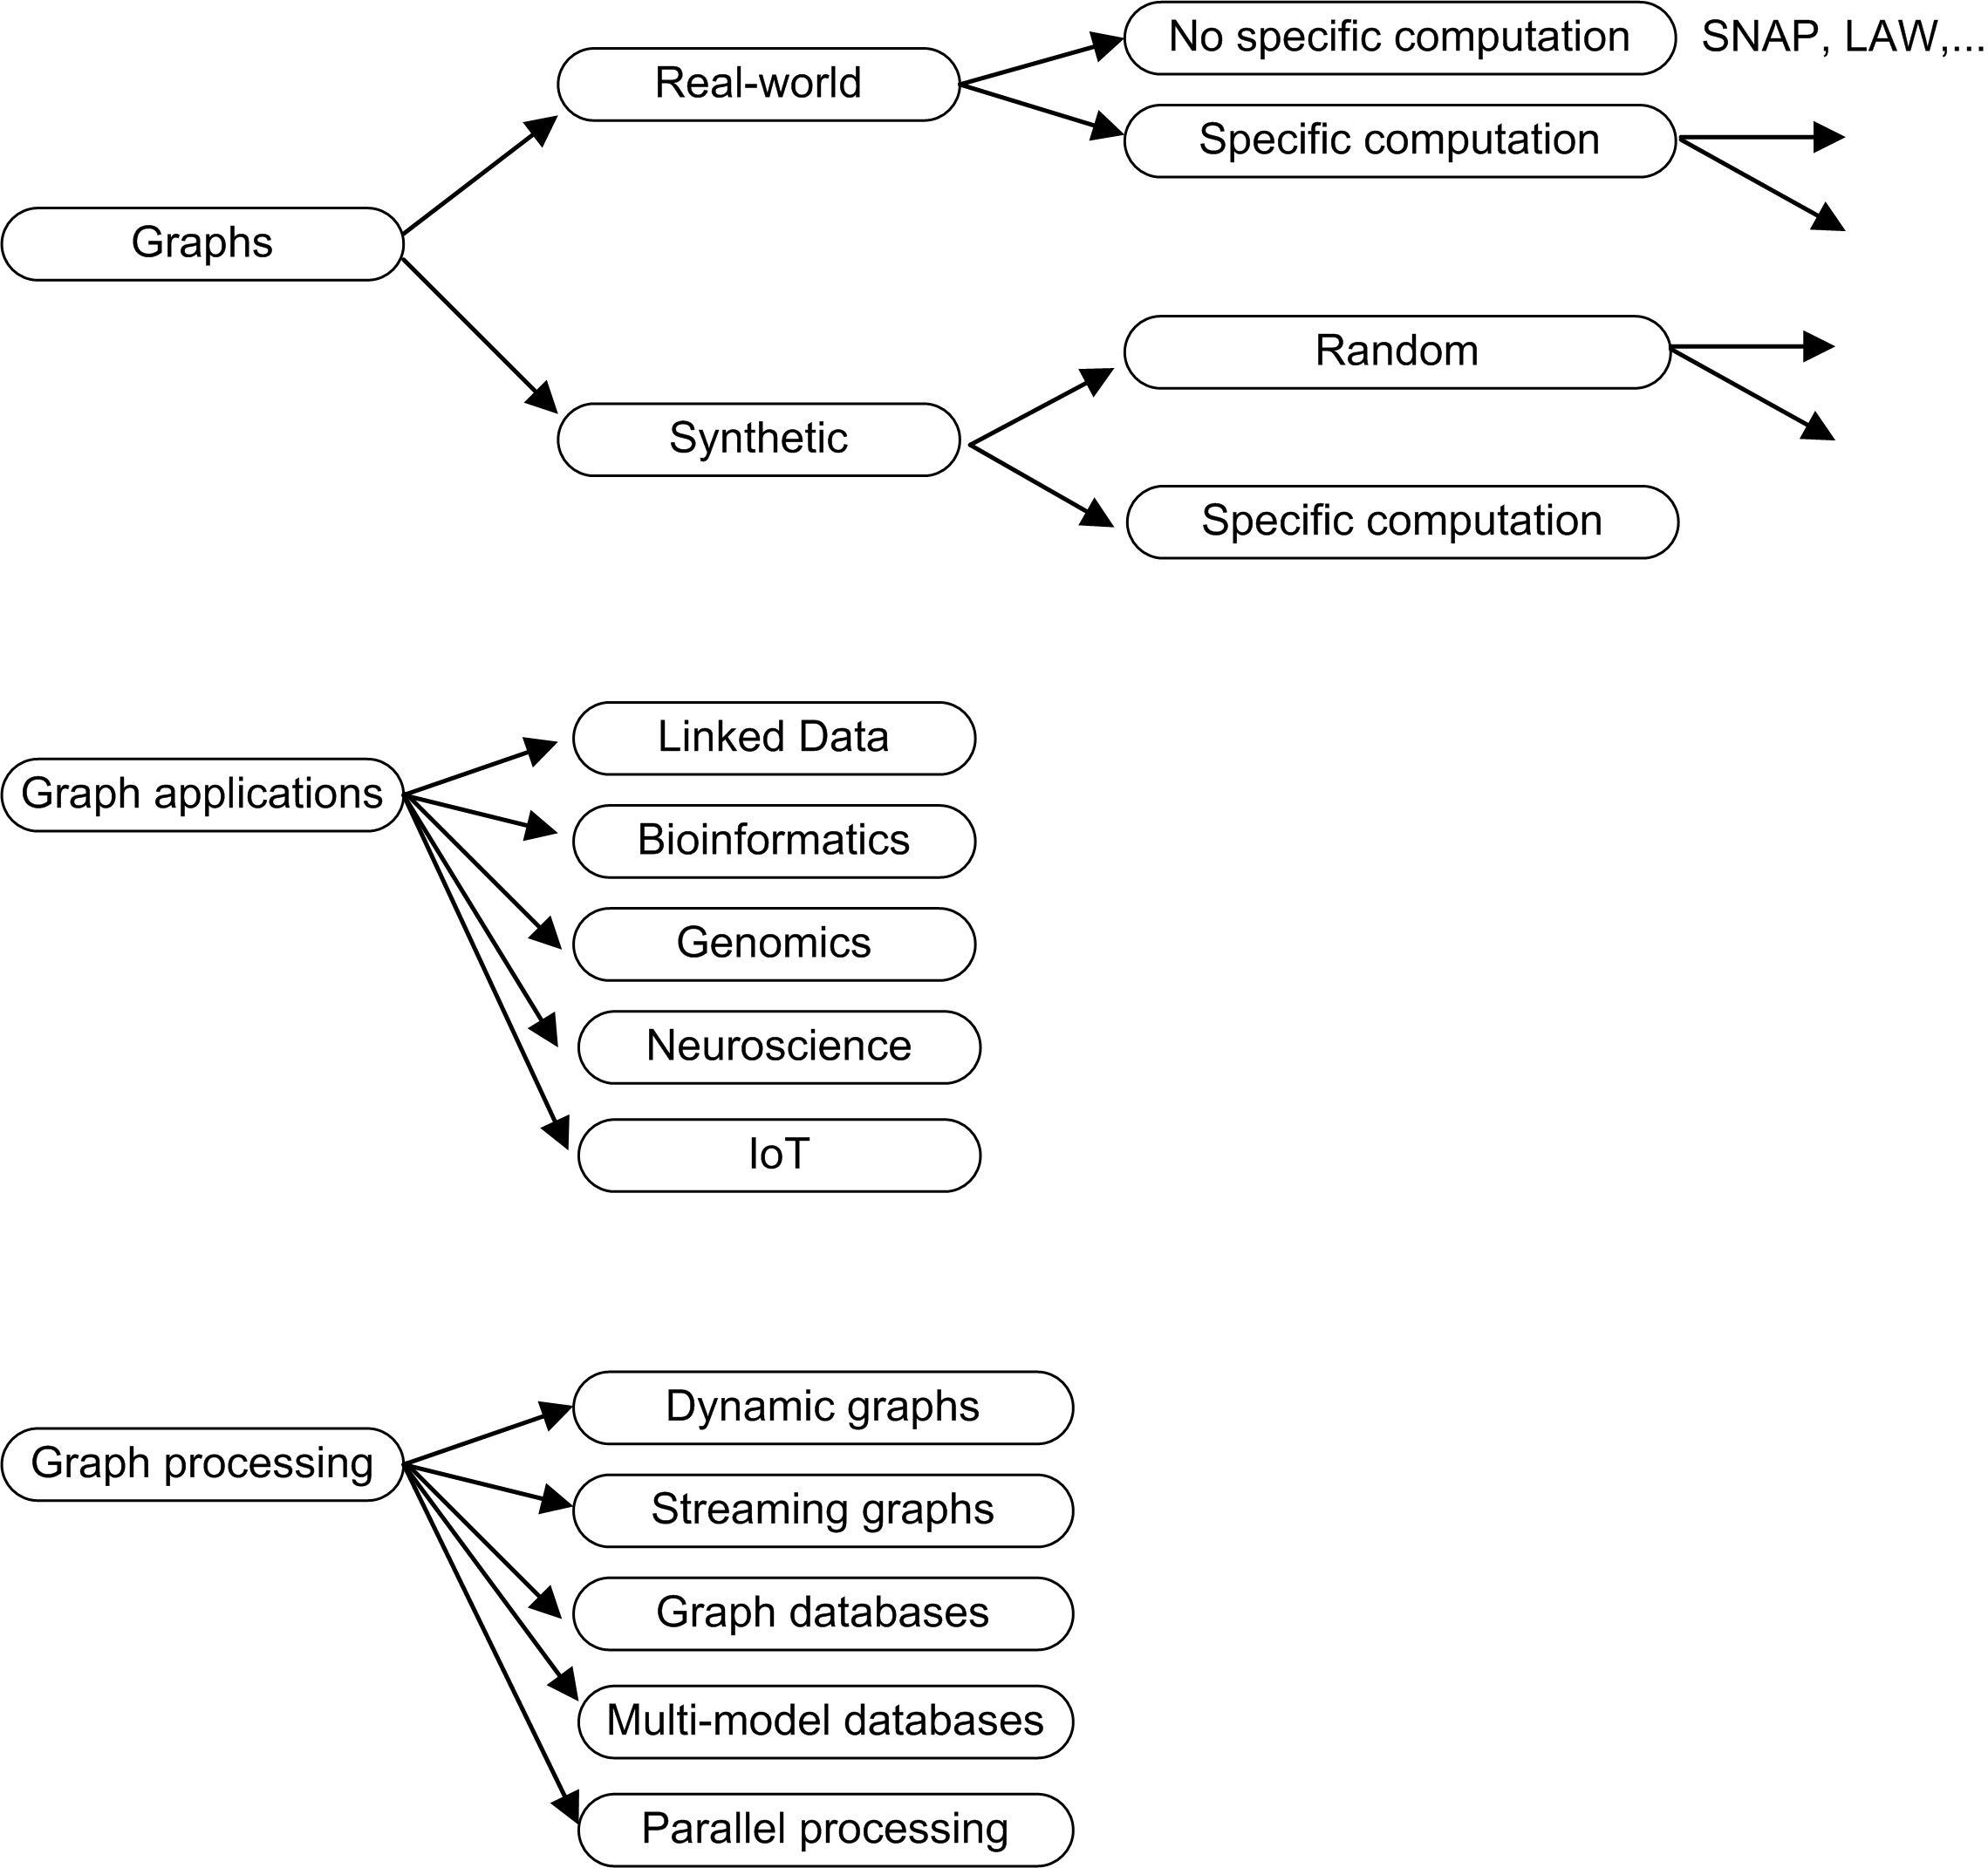
\includegraphics[width=0.8\textwidth]{classification.png}
%\caption{Classification of graph data generators}
%\label{fig:classification}
%\end{figure}

\subsection{Classification}

At first we classify the generators on the basis of the respective application domains or user communities. In particular we distinguish (1) general graphs, (2) Semantic Web, (3) graph databases, (4) social networks, (5) graph analytics, and (6) graph data steaming. The selected classes are not rigorously defined (e.g., they are not disjoint as we will show later), but they correspond to the currently most active research areas. Thus we believe that they form a natural first acquaintance for the reader.

In Tables~\ref{tab:comparisonCharacteristicsA},~\ref{tab:comparisonCharacteristicsB}   we overview the key characteristics of the data generators clustered according to the respective application domains.\footnote{``GDBs'' stands for graph databases, ``SNs'' stands for social networks, ``An.'' stands for graph analytics, ``St.'' stands for graph streaming. Value ``$-$'' means that the information is not available or relevant.} In particular, we show:

\begin{itemize}
\item Characteristics of the \textbf{domain} -- its \textit{type} (fixed, specified using a schema, or extracted from input data) and the particular \textit{target} domain, or, in case of a generic tool, the chosen sample domain,
\item Characteristics of \textit{read}/\textit{update} \textbf{operations} (if provided), i.e., whether the set of operations is fixed/generated, if it involves operation mixes (i.e., sets/sequences of operations), or if templates of operations are supported.
\item Key \textbf{configuration} options:
  \begin{itemize}
    \item whether the generator deals only with structure, or also with \textit{properties} of the graph (Y/N feature),
    \item supported types of \textit{distributions} used for generating of the data,
    \item \textit{output format} of the produced graph, and
    \item  whether the generator is \textit{distributed} and thus enables more efficient data generation (Y/N feature).
  \end{itemize}
\end{itemize}




\begin{sidewaystable}
\scriptsize
\centering
\tbl{Key characteristics of the generators (part A)} {
\begin{tabular}{| c | p{2.2cm} | p{2cm} |  p{2.2cm} | l |  l | l | p{3cm} | p{1.4cm} | l | }
 \hline
           &   & \multicolumn{2}{c}{\textbf{Domain}}
               & \multicolumn{2}{|c|}{\textbf{Operations}}
               & \multicolumn{4}{c|}{\textbf{Configuration}}
               \\ \hline
           &  \textbf{Generator}
               & \textbf{Type}
               & \textbf{Target / sample}
               & \textbf{Read}
               & \textbf{Update}
               & \textbf{\rot{Properties}}
               & \textbf{Distributions}
			   & \textbf{Output}
               & \textbf{\rot{Distributed\ }}
               \\ \hline
\hline   % ====================== general graphs
\multirow{8}{*}{\rot{\textbf{General}}}
  & \cite{barabasi1999emergence} & -- & N & Y & N & Y & power-law & edge-list &  N  \\
\cline{2-10}
   & R-MAt & -- & N & Y & N & Y & power-law & edge-list &  N  \\
\cline{2-10}
  & GraphGen & -- & N & Y & N & Y& user-defined  & JSON & N   \\
\cline{2-10}
  & Graph 500  & -- & various domains & Y & N & Y & power-law & edge-list &  Y  \\
\cline{2-10}
  & BTER & -- & N &   N &  & N & user-defined & edge-list & Y  \\
\cline{2-10}
  & Darwini & -- & N &   N &  & N & user-defined &  edge-list & Y   \\
%  & Watts-Strogatz~\cite{watts1998collective} & fixed & & Y & N & Y &  & &  N  \\
%\cline{2-10}
\hline
\hline %  ======================  Semantic web
\multirow{20}{*}{\rot{\textbf{Semantic web}}}
 & LUBM & fixed & university  & fixed & N & Y & random (LCG) &  RDF & N   \\
\cline{2-10}
 & LBBM & extracted & Lehigh university BibTeX  & N & N & Y & Monte Carlo &  RDF & N   \\
\cline{2-10}
 & UOBM & fixed & university  & fixed & N & Y & random &  RDF & N   \\
\cline{2-10}
 & IIMB & fixed & movies  & N & N & Y & random &  RDF & N   \\
\cline{2-10}
 & BSBM & fixed & e-commerce  & fixed & N & Y & mostly normal &  RDF, relational & N   \\
\cline{2-10}
 & SP$^2$Bench & fixed & DBLP  & fixed & N & Y & based on DBLP  & RDF & N   \\
\cline{2-10}
 & \cite{Duan:2011:AOC:1989323.1989340} & extracted & -- & N & Y &N & -- &  RDF & N    \\
\cline{2-10}
 & DBPSB & extracted & DBpedia &  templates & N & Y & random &  RDF & N   \\
\cline{2-10}
 & LODIB & fixed & e-commerce &  N & N & Y & 44 types &  RDF & N   \\
\cline{2-10}
 & SIB & fixed & social network &  mixes & mix & Y & from real-world data &  RDF & N   \\
\cline{2-10}
 & Geographica & fixed & OpenStreetMap  & fixed + templates  & N & Y & -- &  RDF & N   \\
\cline{2-10}
 & WatDiv & schema-driven & user-defined  & templates & N & Y & uniform, normal, Zipfian &  RDF & N   \\
\cline{2-10}
 & RBench & extracted & DBLP, Yago  & templates & N & Y & from real-world data &  RDF & N  \\
\cline{2-10}
 & LDBC SPB & fixed & media  & mixes & N & Y & power law, skewed values, value correlation &  RDF & N  \\
\cline{2-10}
 & LinkGen & schema-driven & user-defined & templates & Y  & N & Gaussian, Zipfian & RDF & N\\
\hline
\end{tabular} }
\label{tab:comparisonCharacteristicsA}
\end{sidewaystable}

\begin{sidewaystable}
\scriptsize
\centering
\tbl{Key characteristics of the generators (part B)} {
\begin{tabular}{| c | p{2.2cm}| p{2cm} |  p{2.2cm} | l |  l | l | p{3cm} | p{1.4cm} | l | }
 \hline
           &   & \multicolumn{2}{c}{\textbf{Domain}}
               & \multicolumn{2}{|c|}{\textbf{Operations}}
               & \multicolumn{4}{c|}{\textbf{Configuration}}
               \\ \hline
           &  \textbf{Generator}
               & \textbf{Type}
               & \textbf{Target / sample}
               & \textbf{Read}
               & \textbf{Update}
               & \textbf{\rot{Properties}}
               & \textbf{Distributions}
			   & \textbf{Output}
               & \textbf{\rot{Distributed\ }}
               \\ \hline
\hline  % ======================  graph databases
\multirow{7}{*}{\rot{\textbf{GDBs}}}
  & XGDBench & fixed  & social network  & fixed & Y & Y & power-law &  MAG &  Y  \\
\cline{2-10}
  & gMark & schema-driven &  user-defined  & generated &  N  & Y & uniform, normal, Zipfian &  N-triples & N    \\
\cline{2-10}
  & graphGen & pattern-driven & user-defined  & -- & -- & Y & -- &  property graphs & N   \\
\hline
\hline %  ======================   social networks
\multirow{11}{*}{\rot{\textbf{SNs}}}
 & \cite{Barrett:2009:GAL:1995456.1995598} & fixed & social network & N & N & Y & simulation-driven & impl. not available &  -- \\
\cline{2-10}
 & \cite{Yao2011} & fixed & social network & N & N & N & power-law & impl. not available & --  \\
\cline{2-10}
 & LinkBench & fixed & social network & Y & Y & Y & Facebook & impl. not available & -- \\
\cline{2-10}
 & S3G2 & fixed & social network  & N & N  & Y & Facebook  & CSV, RDF & Y   \\
\cline{2-10}
 & \cite{Sukthankar-SocialInfo2014} & schema-driven & social-network & N & N & Y & power-law & CSV & N   \\
\cline{2-10}
 & LDBC SNB  & fixed & social network &  generated & Y  & Y & Facebook &  CSV, RDF & Y     \\
\cline{2-10}
  & \cite{Nettleton2016} & schema-driven & social network & N & N & Y & power-law & impl. not available & --  \\
%\cline{2-10}
% & SNG  & Y & Y &   N &  & Y & power-law & ? &  ?   \\
%\cline{2-10}
% & Forest Fire  & N & Y   & N &  & N & power-law &  ? & N   \\
\hline
\hline   % ======================   graph analytics
\multirow{3}{*}{\rot{\textbf{Ana.}}}
  & HPC Scalable Graph Analysis & fixed & & Y & N& N& uniform &edge-list & N   \\
\cline{2-10}
  & Graphalytics & extracted & social network & Y& N& N & power law & CSV, RDF & N   \\
\hline
\hline   %  ======================  streaming
\multirow{2}{*}{\rot{\textbf{St.}}}
  & S2Gen & schema-driven & social network & Y & N & N & user-defined & RDF & N     \\
\cline{2-10}
  & RSPLab & schema-driven & agnostic & Y & Y & N & user-defined & RDF & N     \\
%\cline{2-10}
%  & & & & & & & &  &   \\
\hline
\end{tabular} }
\label{tab:comparisonCharacteristicsB}
\end{sidewaystable}

\paragraph{Number of Generators, Size of the Data}
As we can see, the biggest set of available generators can be found in the Semantic Web application domain, probably due to its recent popularity and a number of research groups dealing with this topic. On the other hand, none of these generators is natively implemented in a distributed manner and thus generating  output at the Big Data scale. Linked Open Data (LOD) are expected to be large in general, however this is the case of the whole \emph{LOD Cloud}\footnote{\url{https://lod-cloud.net/}}, but not necessarily of the particular data sets forming it.

The second large group of generators also corresponds to a popular application domain -- social networks. In this case the size of the output graph is important if we require realistic features of the output. However, most of the proposals do not provide an implementation and, thus, this aspect cannot be discussed reliably.

In case of the other application-specific domains the amount of generators is not that significant. As we will show in Section~\ref{sec:overlapping}, the situation is not that critical. Some of the application-specific generators can be re-used also in other application domains or the general graph generators can be used as well.

\paragraph{Domain}

If we consider the features of the domain of the generators, in most cases it is expectably fixed which is the simplest option and which may, however, also mean that the generator focuses on other complex aspects of the output. Except for general graphs without any domain, in all other cases we can find a representative with schema-driven domain or a domain extracted from sample data. In the group of generators for graph databases we can see two special cases -- gMark ... \TODO{Explain schema-driven (internal schema)} and graphGen ... \TODO{Explain pattern-driven
(Cypher schema)}.

The particular target (in case of fixed) or sample (in case of schema-driven or extracted) domains do not provide very rich areas. They either correspond to the respective application domains (like in the case of social networks), or they are based on well-known and commonly used data sets (such as, e.g., DBLP or DBpedia). This narrow scope can can, however, be solved by using one of the representatives with schema-driven or extracted target domains.

\paragraph{Operations}
While the read operations are quite commonly provided, in case of updates

\TODO{...}

\paragraph{Configuration}

\TODO{...}

\subsection{Overlapping}
\label{sec:overlapping}

As we have mentioned, the basic classification that we have used in this paper
is  based on a relatively vague division of the generators on the basis of the
current application domains or research areas. In addition, some of the
generators are either general or have features applicable in other domains. So
the classes can overlap, as depicted in Table~\ref{tab:overlapping}.

\begin{table}[h]
\scriptsize
\centering
\tbl{Overlapping of classes of generators} {
\begin{tabular}{| c | l | l | l | l | l | l | l | }
 \hline
           &  \textbf{Generator}
               & \textbf{\rot{General}}
               & \textbf{\rot{Semantic Web}}
               & \textbf{\rot{Graph databases\ }}
               & \textbf{\rot{Social networks}}
               & \textbf{\rot{Analytics}}
               & \textbf{\rot{Steaming}}
               \\ \hline
\hline   % ====================== general graphs
\multirow{6}{*}{\rot{\textbf{General}}}
  & \cite{barabasi1999emergence} & {\bf x} & & & & x & \\
\cline{2-8}
   & R-MAt    & {\bf x} & & & & x & \\
\cline{2-8}
  & GraphGen  & {\bf x} & & x & & & \\
\cline{2-8}
  & Graph 500 & {\bf x} & & & & x & \\
\cline{2-8}
  & BTER      & {\bf x} & & & & & \\
\cline{2-8}
  & Darwini   & {\bf x} & & & & & \\
\hline
\hline %  ======================  Semantic web
\multirow{15}{*}{\rot{\textbf{Semantic web}}}
 & LUBM  & & {\bf x} & & & & \\
\cline{2-8}
 & LBBM  & & {\bf x} & & & & \\
\cline{2-8}
 & UOBM  & & {\bf x} & & & & \\
\cline{2-8}
 & IIMB & & {\bf x} & & & & \\
\cline{2-8}
 & BSBM & & {\bf x} & & & & \\
\cline{2-8}
 & SP$^2$Bench & & {\bf x} & & & & \\
\cline{2-8}
 & \cite{Duan:2011:AOC:1989323.1989340} & & {\bf x} & & & & \\
\cline{2-8}
 & DBPSB & & {\bf x} & & & & \\
\cline{2-8}
 & LODIB & & {\bf x} & & & & \\
\cline{2-8}
 & SIB & & {\bf x} & & & & \\
\cline{2-8}
 & Geographica & & {\bf x} & & & & \\
\cline{2-8}
 & WatDiv & & {\bf x} & & & & \\
\cline{2-8}
 & RBench & & {\bf x} & & & & \\
\cline{2-8}
 & LDBC SPB & & {\bf x} & & & & \\
\cline{2-8}
 & LinkGen & & {\bf x} & & & & \\
\hline
\hline  % ======================  graph databases
\multirow{3}{*}{\rot{\textbf{GDBs}}}
  & XGDBench & & & {\bf x} & x & & \\
\cline{2-8}
  & gMark & & x & {\bf x} & x & & \\
\cline{2-8}
  & graphGen & & & {\bf x} & & & \\
\hline
\hline %  ======================   social networks
\multirow{7}{*}{\rot{\textbf{SNs}}}
 & \cite{Barrett:2009:GAL:1995456.1995598} & & & & {\bf x} & & \\
\cline{2-8}
 & \cite{Yao2011}  & & & & {\bf x} & & \\
\cline{2-8}
 & LinkBench  & & & x & {\bf x} & & \\
\cline{2-8}
 & S3G2  & & x & x & {\bf x} & & \\
\cline{2-8}
 & \cite{Sukthankar-SocialInfo2014}  & & & & {\bf x} & & \\
\cline{2-8}
 & LDBC SNB   & & x & x & {\bf x} & & \\
\cline{2-8}
  & \cite{Nettleton2016}  & & & & {\bf x} & & \\
\hline
\hline   % ======================   graph analytics
\multirow{2}{*}{\rot{\textbf{An.}}}
  & HPC Scalable Graph Analysis  & & & & & {\bf x} & \\
\cline{2-8}
  & Graphalytics & & & & & {\bf x} & \\
\hline
\hline   %  ======================  streaming
\multirow{2}{*}{\rot{\textbf{St.}}}
  & S2Gen & & & & & & {\bf x}\\
\cline{2-8}
  & RSPLab & & & & & & {\bf x} \\
%\cline{2-8}
%  & & & & & & \\
\hline
\end{tabular} }
\label{tab:overlapping}
\end{table}

For example, many general or domain-agnostic graph generators such as the
preferential attachment, RMAT or Graph500, are typically used to test graph
analytics frameworks when large real graphs are not available. Actually,
Graphalytics uses RMAT as one as its graph generators for benchmarking graph
analytics.

Similarly, some social network graph generators such as LDBC-SNB, S3G2 or
LinkBench, can be used to test graph databases. In the case of the first two,
even though they are designed not to be specific to any type of technology,
the graph databases are their main target.  Additionally, they also provide serializers for
RDF, thus they can also be used to test RDF systems.

In the case of LinkBench, nothing prevents the user to load the generated graph
in a graph database (Facebook uses MySQL in that paper) to
test a workload similar to Facebook and extend and complement it with more
graph queries like those in LDBC-SNB.

\TODO{...}

\section{Classification of Graph Data Generators}
\label{sec:classification}

The graph data generators can be classified according to distinct criteria. For example, paper~\cite{DBLP:conf/sdm/ChakrabartiZF04} introduces two categories:

\begin{itemize}
  \item \emph{Degree-based generators}: Given a degree distribution (typically following a power law), these generators (e.g., Barabasi-Albert model~\cite{Barabasi99emergenceScaling}) try to find a graph that matches it, but without giving any insights about the graph or trying to match other criteria (like, e.g., small diameter, eigenvalues etc.).
  \item \emph{Procedural generators}: These generators (e.g., R-MAT~\cite{DBLP:conf/sdm/ChakrabartiZF04}) try to find simple mechanisms to generate graphs that match a property of the real graphs and, typically, the power law degree distribution.
\end{itemize}

Paper~\cite{Chakrabarti:2006:GML:1132952.1132954} introduces five categories of graph models (examples are further described below):
\begin{itemize}
  \item \emph{Random graph models} (e.g., Erd\"{o}s-R\'{e}nyi~\cite{Erdos:1960}) generated by a random process,
  \item \emph{Preferential attachment models} (e.g., Barabasi-Albert model) which try to model the power law from the preferential attachment viewpoint,
  \item \emph{Optimization-based models} (e.g., HOT model~\cite{PhysRevLett.84.2529}) resulting from the idea that power laws can result from resource optimizations and tolerance to risks,
  \item \emph{Tensor-based models} (e.g., R-MAT) targeting a trade-off between low number of model parameters and efficiency, and
  \item \emph{Internet-specific models} corresponding to hybrids using ideas from the other categories in order to suit the specific features of the graphs.
\end{itemize}

\paragraph{Erd\"{o}s-R\'{e}nyi} One of the first and still very popular approaches with lots of variations and modifications is the random graph model proposed in~\cite{Erdos:1960}. Given a positive integer $n$ and a probability value $0 \leq p \leq 1$, the graph $G(n,p)$ is an undirected graph on $n$ vertices whose edges are chosen s.t. for all pairs of vertices $u,v$ there is an edge $(u,v)$ with probability $p$.

\paragraph{Barabasi-Albert} The Barabasi-Albert (BA) model~\cite{Barabasi99emergenceScaling} proposes that structure emerges in network topologies as the result of two processes -- growth and preferential attachment. The BA model starts with a small set of nodes and grows the network as nodes and edges are added over time. Preferential attachment is based on the idea that the probability of connecting to a node is proportional to the current degree of that node (i.e., ``the rich get richer'').

\paragraph{HOT} The highly optimized tolerance (HOT)~\cite{PhysRevLett.84.2529} model is introduced  using a ``forest fire'' example as follows: Suppose we have a forest which is prone to forest fires. Each portion of the forest has a different chance of starting the fire. We wish to minimize the damage by assigning (a limited amount of) resources such as firebreaks at different positions in the forest. More precisely, we have $n$ possible events, each with an associated probability $p_i, 1 \le i \le n$. Each event can lead to some loss $l_i$, which is a function of the resources $r_i$ allocated for that event $(l_i = f (r_i))$, whose total number is limited ($\sum_i r_i \le R$ for some given $R$). The aim is to minimize the expected cost $\sum_i p_i l_i$. The authors show that resource placement is related to the probability distribution $p_i$ by a power law and the probability of events which cause a loss greater than some value $k$ is related to $k$ by a power law too.


\paragraph{R-MAT} The R-MAT (Recursive MATrix)~\cite{DBLP:conf/sdm/ChakrabartiZF04} model can be used to create graphs with community structure, power law degree distributions, and a small diameter. It generates weighted, directed and bipartite graphs. Graph generation is modeled with a matrix recursion procedure in which the adjacency matrix (empty at the beginning) is recursively subdivided into four equal-sized partitions and edges are distributed across the partitions with unequal probabilities.
\\



...


%~\cite{Gray:1992:BHD:530588}

Ideas to describe:

\begin{itemize}
  \item Domain-specific - predefined schema and domain knowledge - vs. application-specific~\cite{Tay2011}
  \item Use-case driven
  \item Query-centric vs. workload-driven~\cite{gMark}
  \item Language-specific (the document and query design is specifically laid out to test common language constructs, operator constellations, and data access patterns)~\cite{Schmidt2010}
  \item Application benchmarks attempt to predict the behaviour of a system on
certain classes of application by testing an example (or select examples) of that
class.
  \item Analytical benchmarks attempt to determine the presence or absence of cer-
tain performance related features, e.g., the presence of a query optimiser.
\end{itemize}

...

In Figure~\ref{fig:classification} ...

\begin{figure}
\centering
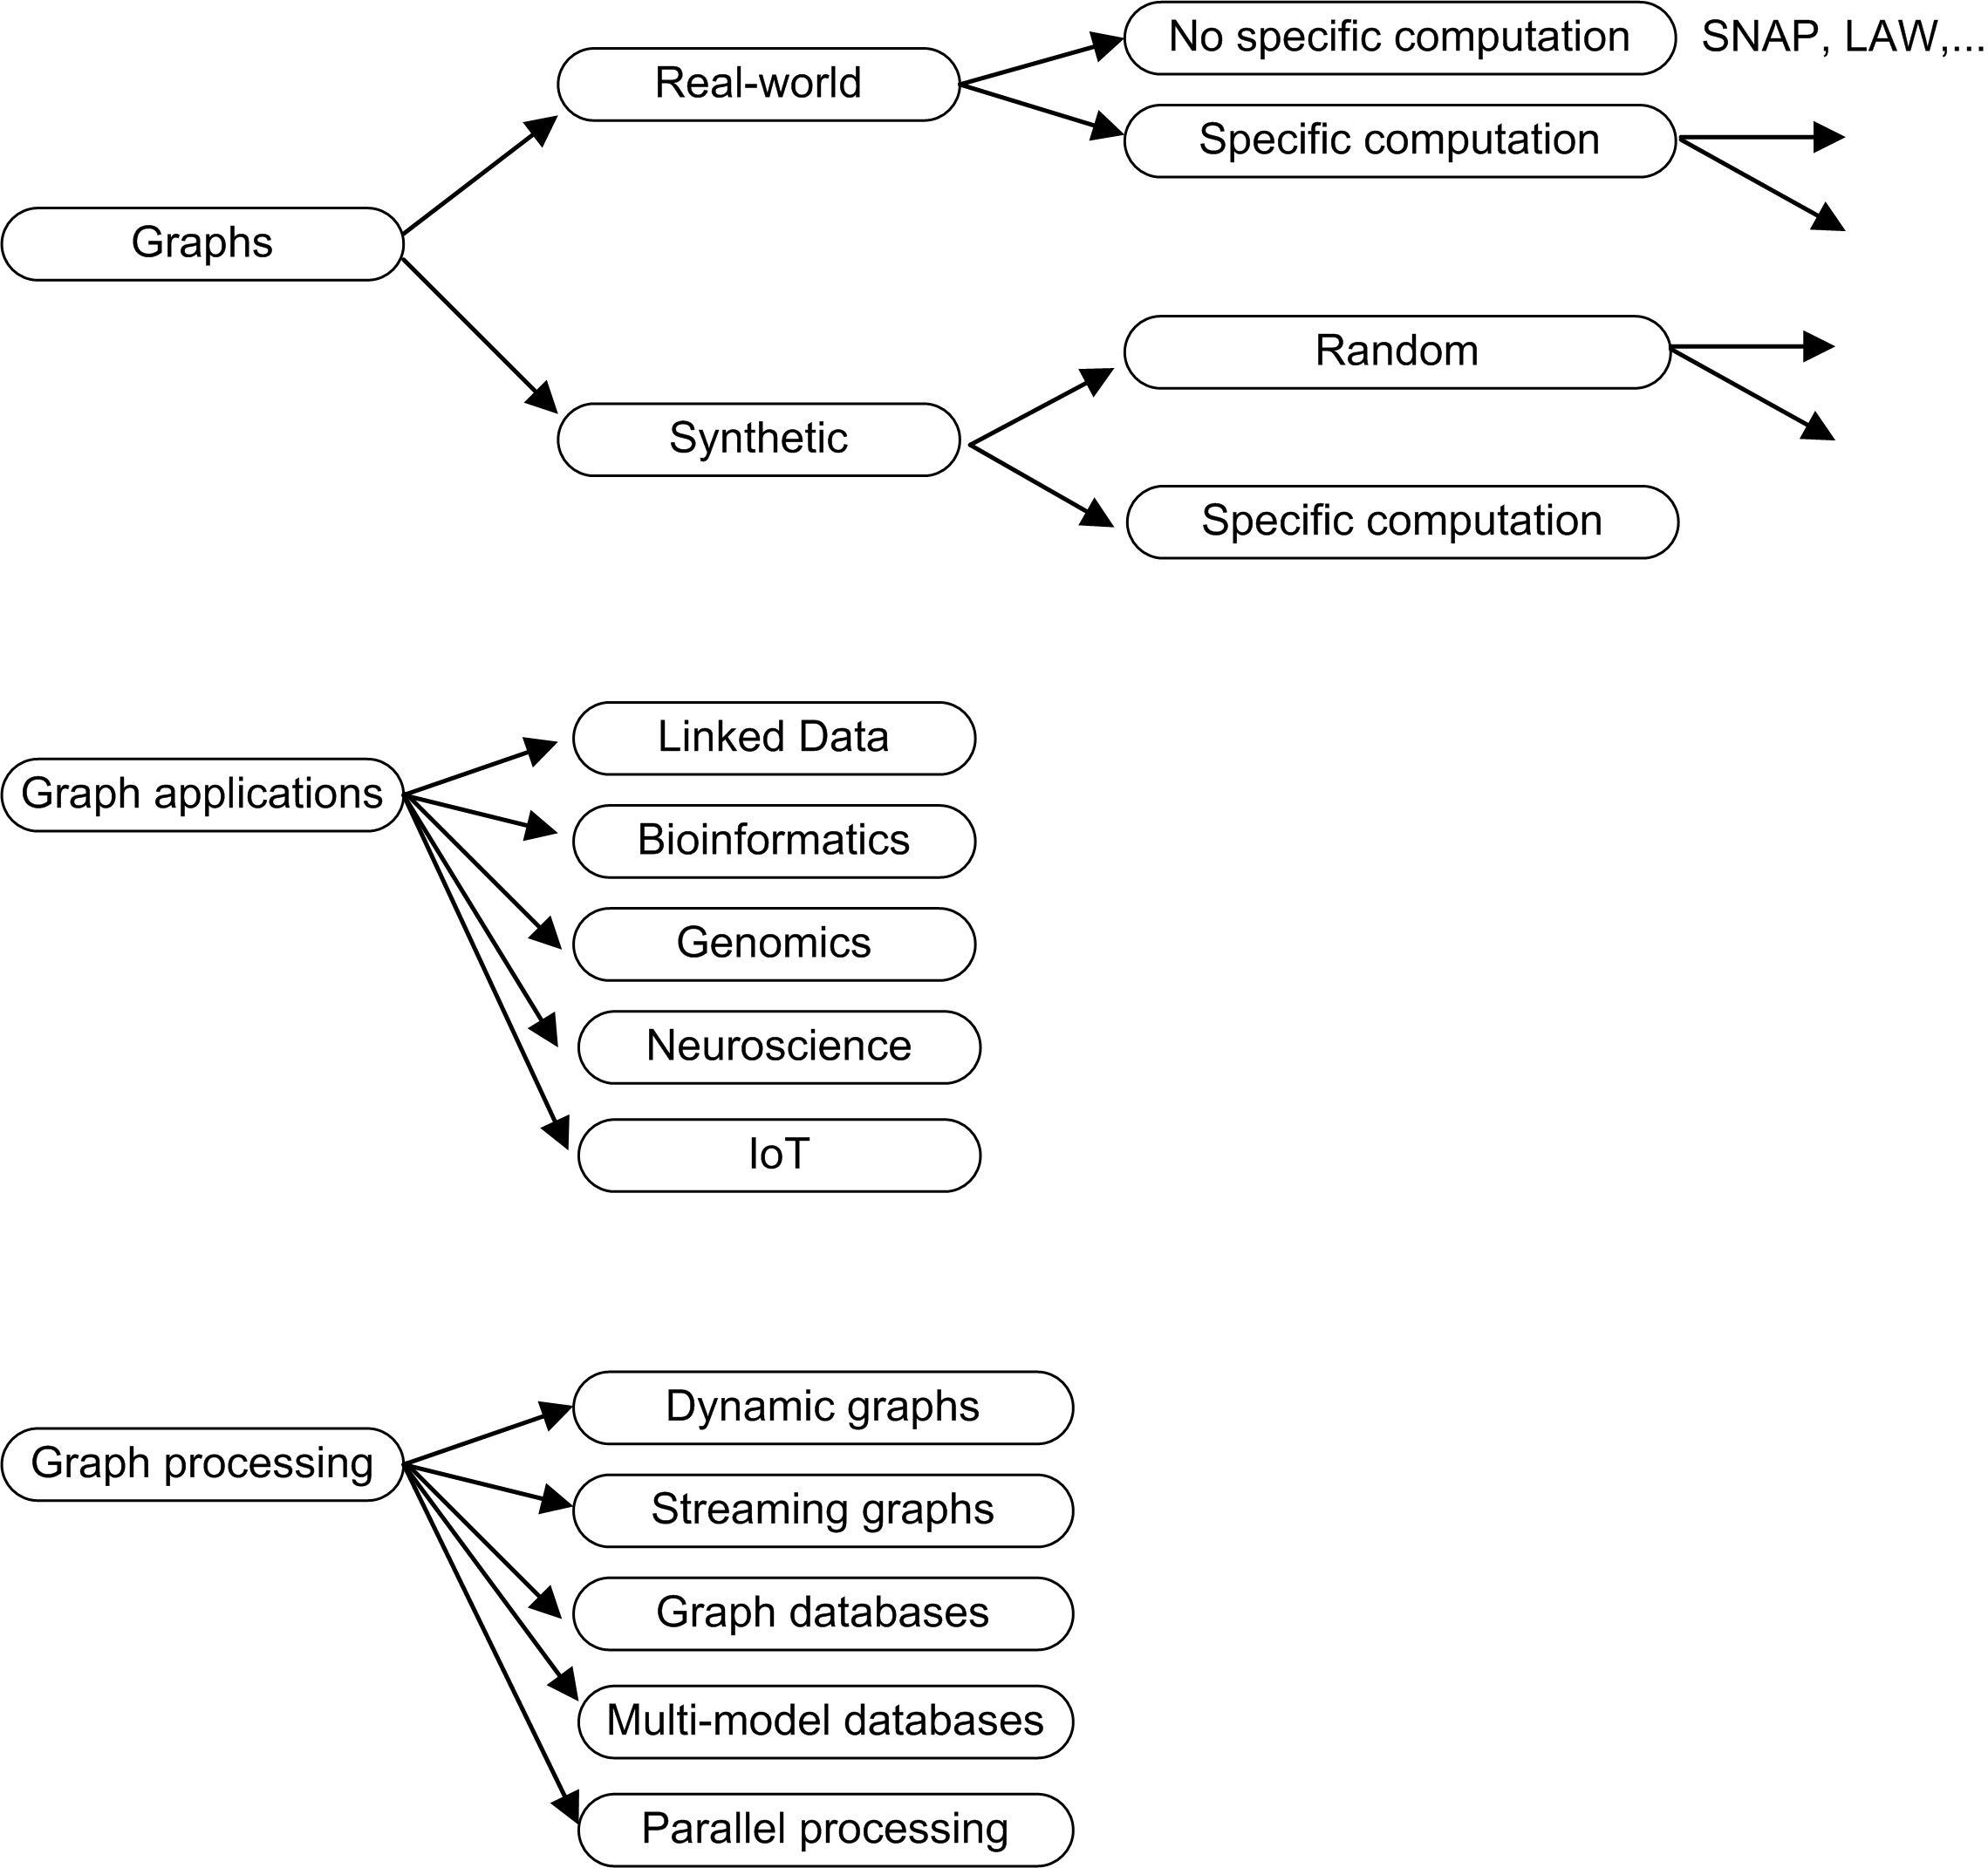
\includegraphics[width=0.8\textwidth]{classification.png}
\caption{Classification of graph data generators}
\label{fig:classification}
\end{figure}

\section{Graph Data Generators}
\label{sec:generators}

In this section, we discuss the various graph data generators based on the classification introduced before in more detail. For each category, we first describe the key features of each of the representative examples and summarize their strengths and weaknesses. The goal is to offer a detailed information about each of the tools in the context of its competitors from the same domain.


\subsection{General Graphs}
\label{sec:generators_general}

We start by focusing on approaches that have been designed for dealing with the generation of general graph
data that is not aimed at a particular application domain. Currently, there exists a
number of tools which involve a kind of general graph data generator, such as
gtools from projects nauty and Traces~\cite{gtools} or the Stanford
GraphBase~\cite{GraphBase}. We, however, focus on primarily
generating/benchmarking projects targeting the Big Data world.


\paragraph {Preferential Attachment} Barabasi and Albert~\cite{Barabasi99emergenceScaling} introduced a graph generation model that relies on two main mechanisms. The first mechanism is continuously expanding the graphs by adding new vertices. The second mechanism is to preferentially attach the new vertices   to the nodes/regions that are already well connected. So, in this approach, the generation of large graphs is governed by standard, robust self-organizing mechanisms that go beyond the characteristics of individual applications.

\paragraph {R-Mat} (\emph{R}ecursive \emph{Mat}rix) R-Mat is a procedural synthetic graph generator which is designed to generate power-law degree
distributions~\cite{DBLP:conf/sdm/ChakrabartiZF04}.
The generator is recursive and uses only a small number of parameters.
In principle, the strategy of this generator is to find simple mechanisms to generate graphs that match
the properties of the real graphs. In particular, the design goals of R-Mat is to generate graphs that match the degree distributions, imitate a community structure and have a small diameter. R-Mat can generate weighted, directed and bipartite graphs.

\paragraph{GraphGen} For the purpose of testing the scalability of an indexing
technique called FG-index~\cite{Cheng:2007:FTV:1247480.1247574} on the size of the
database of graphs, their average size and average density, the authors have
also implemented a synthetic generator called
GraphGen~\footnote{https://www.cse.ust.hk/graphgen/}. It is
based on the IBM synthetic data generation code for associations and sequential
patterns\footnote{From 1996, no longer available at
\url{http://www.almaden.ibm.com/cs/projects/iis/hdb/Projects/data
mining/mining.shtml}}. GraphGen creates a collection of labeled, undirected and
connected graphs which focuses on the performance evaluation of frequent subgraph mining
algorithms and graph query processing algorithms. The result is represented as a
list of graphs, each consisting of a list of nodes and a list of edges.




\paragraph{Graph 500 Benchmark} The Graph 500 Benchmark~\cite{Graph500} includes
a scalable data generator which produces weighted, undirected graph as a list of
edge tuples containing the label of start vertex and end vertex together with a
weight that represents data assigned to the edge. The space of vertex  labels is
the set of integers beginning with 0. The input values required to describe the
graph are (1) scale, i.e., the logarithm base two of the number of vertices, and
(2) edge factor, i.e., the ratio of the graph's edge count to its vertex count
(i.e., half the average degree of a vertex in the graph). The graph generator is
a Kronecker generator similar to R-MAT. The data must not exhibit any locality,
so in the final step the vertex labels and order of edges are randomly shuffled.
The covered operations currently involve BFS; however, the authors intend to
involve also two more types -- optimization (single source shortest path) and
edge-oriented (maximal independent set) -- and five graph-related business areas:
cybersecurity, medical informatics, data enrichment, social networks, and
symbolic networks.

\paragraph{BTER} BTER (Block Two-Level
Erd\"{o}s-R\'{e}ny)~\cite{kolda2014scalable} is a graph generator based on the
creation of multiple Erd\"{o}s-R\'{e}ny graphs with different connection
probabilities  of which they are connected randomly between them. As the main feature, BTER is able
to reproduce input degree distributions and average clustering
coefficient per degree values. The generator starts by grouping the vertices
by degree $d$, and forming groups of size $d+1$ of nodes with degree $d$. Then, these
groups are assigned an internal edge probability in order to match the observed
average clustering coefficient of the nodes of such degree. Based on this
probability, for each node, the excess degree (i.e, the degree that in
expectation will not be realized internally in the group) is computed and used to connect
nodes from different groups at random. The authors describe a highly scalable
MapReduce based implementation that is capable of generating large graphs (with
billions of nodes) in a reasonable amounts of time.

\paragraph{Darwini} Darwini~\cite{edunov2016darwini} is an extension of BTER
designed to run on Vertex Centric computing frameworks like
Pregel~\cite{malewicz2010pregel} or Apache Giraph~\cite{ching2015one}, with the
additional feature that it is more accurate when reproducing the clustering
coefficient of the input graph. Instead of just focusing on the average
clustering coefficient for each degree, Darwini is able to model the clustering
coefficient distribution per degree. It achieves this by grouping the vertices
of the graph into buckets by the expected number of closed triangles that they need
to close in order to attain the expected clustering coefficient, which is
sampled from the input distributions. Then, the vertices in each bucket are
connected randomly with a probability that would produce the expected 
desired number of triangles for such bucket. Then, as in BTER, the excess degree
is used to connect the different buckets. The authors report that Darwini is
able to generate graphs with billions and even trillions of edges.

%\paragraph{gtools} Projects nauty and Traces~\cite{gtools} are programs for
%computing automorphism groups of graphs and digraphs~\cite{McKay201494}; they
%can also produce a canonical label. In the respective package there is also
%suite of programs called gtools which involve generators for non-isomorphic
%graphs, bipartite graphs, digraphs, and multigraphs.





\subsection{Semantic Web}
\label{sec:generators_LinkedData}
With the dawn of the concept of Linked Data it is a natural development that there would emerge respective benchmarks involving both synthetic data and real-world data sets  sets with real-world characteristics. The used data sets correspond to RDF representation of relational-like data~\cite{Guo2005158,Bizer09theberlin}, social network-like data~\cite{Schmidt2010}, or specific and significantly more complex data structures such as biological data~\cite{Wu2014}. In this section, we provide an overview of benchmarking systems involving a kind of graph-based RDF data generator or data modifier. %Other types of systems or particular results can be found, e.g., at~\cite{RdfStoreBenchmarking}.

\iffalse
Considering the Big Data world, the Linked Data in general definitely belong to this group since we assume that the Linked (Open) Data Sets form a common Linked Open Data cloud\footnote{\url{http://lod-cloud.net/}}. On the other hand, the particular data sets can be relatively small.
\fi

\paragraph{LUBM} The use-case driven Lehigh University Benchmark (LUBM)\footnote{\url{http://swat.cse.lehigh.edu/projects/lubm/}} considers the university domain. The ontology defines 43 classes and 32 properties~\cite{Guo2005158}. In addition, the LUBM benchmark provides 14 test queries. In particular, the benchmark focuses on \emph{extensional} queries, i.e., queries which target the particular data instances of the ontology, as an opposite to \emph{intentional} queries, i.e., queries which target properties and classes of the ontology. The Univ-Bench Artificial  (UBA) data generator features repeatable and random  data generation (exploiting classical linear congruential generator, LCG, of numbers). In particular, the data which is produced by the generator are assigned zero-based indexes (i.e., the first university is named \emph{University0} and so on), thus they are reproducible at any time with the same indexes.  The generator naturally allows to specify a seed for random number generation, along with the desired number of universities, and the starting index of the universities.

An extension of LUBM, the Lehigh BibTeX Benchmark (LBBM)~\cite{Wang2005}, enables generating synthetic data for different ontologies. The data generation process is managed through two main phases: (1) the property-discovery phase, and (2) the data generation phase. LBBM provides a probabilistic model that can emulate the discovered properties of the data of a particular domain and generate synthetic data exhibiting similar properties. A Monte Carlo algorithm is employed to output synthetic data. The approach is demonstrated on the Lehigh University BibTeX ontology which consists of 28 classes along with 80 properties. The LUBM benchmark includes 12 test queries that were designed for the benchmark data. Another extension of LUBM, the University Ontology Benchmark (UOBM)\footnote{\url{https://www.cs.ox.ac.uk/isg/tools/UOBMGenerator/}}, focuses on two aspects: (1) usage of all constructs of OWL Lite and OWL DL~\cite{owl} and (2) lack of necessary links between the generated data which thus form isolated graphs~\cite{Ma:2006:TCO:2094613.2094629}. In the former case the original ontology is replaced by the two types of extended versions from which the user can choose. In the latter case cross-university and cross-department links are added to create a more complex graph.

\paragraph{IIMB} Ferrara et al.~\cite{Ferrara08OM} proposed the ISLab Instance Matching Benchmark (IIMB)\footnote{\url{http://www.ics.forth.gr/isl/BenchmarksTutorial/}} for the problem of instance matching. For any two objects $o_1$ and $o_2$ adhering to the same ontology or to different ontologies, instance matching is specified in the form of a function $Om(o_1, o_2) \rightarrow \{0, 1\}$,  where $o_1$ and $o_2$ are linked to the same real-world object (in which case the function maps to $1$) or $o_1$ and $o_2$ are representing different objects (in which case the function maps to $0$). It targets the domain of movie data which contains 15 named classes, along with 5 object properties and 13 datatype properties. The data are extracted from IMDb\footnote{\url{http://www.imdb.com/}}. The data generator corresponds to a data modifier which simulates differences between the data. In particular it involves data value differences (such as typographical errors or usage of different standard formats, e.g., for names), structural heterogeneity (represented by different levels of depth for properties, diverse aggregation criteria for properties, or missing values specification) and logical heterogeneity (such as instantiation on different subclasses of the same superclass or instantiation on disjoint classes).


\paragraph{BSBM} The Berlin SPARQL Benchmark (BSBM)\footnote{\url{http://wifo5-03.informatik.uni-mannheim.de/bizer/berlinsparqlbenchmark/}}, is centered around an e-commerce application domain with object types such as \emph{Customer}, \emph{Vendor}, \emph{Product} and \emph{Offer} in addition to the relationship among them~\cite{Bizer09theberlin}.
The benchmark provides a workload that has 12 queries with 2 types of query workloads (i.e., 2 sequences of the 12 queries) emulating the navigation pattern and search of a consumer seeking a product. The data generator is capable of producing arbitrarily scalable datasets by controlling the number of products ($n$) as a scale factor.  The scale factor also impacts other data characteristics, such as, e.g., the depth of type hierarchy of products, branching factor, the number of product features,  etc. BSBM can output two representations, i.e. an RDF representation along with a relational representation. Thus, BSBM also defines an SQL~\cite{sql} representation of the queries. This allows comparison of SPARQL~\cite{sparql} results  to be compared against the performance of traditional RDBMSs.


\paragraph{SP$^2$Bench} The SP$^2$Bench\footnote{\url{http://dbis.informatik.uni-freiburg.de/forschung/projekte/SP2B/}} is a language-specific benchmark~\cite{Schmidt2010} which is based on the DBLP dataset. %, so the types involve Person, Inproceedings, Article etc.
The generated datasets follow the key characteristics of the original DBLP dataset. In particular, the data mimics the correlations between entities. All random functions of the generator use a fixed seed that ensures that the data generation process is deterministic. SP$^2$Bench is accompanied by 12 queries covering the various types of operators such as RDF access paths in addition to typical RDF constructs.

%\paragraph{JustBench} ~\cite{Bail:2010:JFO:1940281.1940285} ...




\paragraph{DBPSB} DBpedia SPARQL Benchmark (DBPSB)\footnote{\url{http://aksw.org/Projects/DBPSB.html}} proposed at the University of Leipzig has been designed using workloads that have been issued by humans and applications over existing RDF data~\cite{Morsey2011,Morsey:2012:UBR:2900929.2901031}. In addition, the authors argue that benchmarks like LUBM, BSBM, or SP$^2$Bench resemble relational database benchmarks involving relational data structures with few and homogeneously structured classes, whereas, in reality, RDF datasets are increasingly heterogeneous. For example, DBpedia version 3.6 consists of 289,016 classes of which 275 classes are defined based on the DBpedia ontology. In addition, different data types and object references of the various types are
used in property values. Hence, they presented a universal SPARQL benchmark generation approach which uses a flexible data production mechanism that mimics the input data source. This dataset generation process begins using an input dataset; then multiple datasets with different sizes  are then generated by duplicating all the RDF triples with changing their namespaces.  For generating smaller datasets, an adequate selection of all triples is selected randomly or using a sampling mechanism over the various classes in the dataset. \iffalse The goal of the query analysis and clustering is to detect prototypical queries on the basis of their frequent usage and similarity.\fi The methodology is applied on the DBpedia SPARQL endpoint and a set of 25 SPARQL query templates is derived to cover the frequently used SPARQL features.

\paragraph{LODIB} The Linked Open Data Integration Benchmark (LODIB)\footnote{\url{http://lodib.wbsg.de/}} has been designed with the aim of reflecting the real-world heterogeneities that exist on the Web of Data in order to enable testing of Linked Data translation systems~\cite{DBLP:conf/www/RiveroSBR12}. It provides a catalogue of 15 data translation patterns (e.g., rename class, remove language tag etc.), each of which is a common data translation problem in the context of Linked Data. The benchmark provides a data generator that produces three different synthetic data sets that need to be translated
by the system under test into a single target vocabulary. They  reflect the pattern distribution in analyzed 84 data translation examples from the LOD Cloud. The data sets reflect the same e-commerce scenario used for BSBM.




\paragraph{Geographica} The Geographica benchmark\footnote{\url{http://geographica.di.uoa.gr/}} has been designed to target the area of geospatial data~\cite{DBLP:conf/semweb/GarbisKK13} and respective SPARQL extensions GeoSPARQL~\cite{battle2012enabling} and stSPARQL~\cite{koubarakis2010modeling}. The benchmark involves a real-world workload that uses openly available datasets that cover a range of geometry types (e.g., points, lines, polygons) and  a synthetic workload. In the former case there is a (1) a micro benchmark that evaluates primitive spatial functions (involving 29 queries) and (2) macro benchmark that tests the performance of RDF engines in various application scenarios such as  map exploring and search (consisting of 11 queries). In the latter case of a synthetic workload the generator produces synthetic datasets of different sizes that corresponds to an ontology based on OpenStreetMap  and instantiates query templates. \iffalse The spatial extent of the land ownership dataset constitutes a uniform grid of $n \times n$ hexagons, whereas the size of each dataset is given relatively to $n$.\fi The generated SPARQL query workload is corresponding to spatial selection and spatial joins by instantiating 2 query templates.


\paragraph{WatDiv} The Waterloo SPARQL Diversity Test Suite (WatDiv)\footnote{\url{http://dsg.uwaterloo.ca/watdiv/}} has been designed at the University of Waterloo. It implements stress testing tools that focus on addressing the observation that existing SPARQL benchmarks are not adequate for evaluating systems using a verity of queries and  workloads~\cite{Aluc:2014:DST:2717213.2717229}. The benchmark focuses on two types of query aspects -- structural and data-driven -- and performs a detailed analysis on existing SPARQL benchmarks (LUBM, BSBM, DBPSB, and SP$^2$Bench) using the two classes of query features. The structural features involve triple pattern count, join vertex count, join vertex degree, and join vertex count. The data-driven features involve result cardinality and several types of selectivity. The analysis of the four benchmarks reveals that they are not sufficiently diverse to evaluate the strengths and weaknesses of the various physical design alternatives that have been implemented by the different RDF systems. In particular, WatDiv, provides (1) a data generator which generates scalable datasets according to the WatDiv schema, (2) a query template generator which follows the WatDiv schema and produces a  set of query templates, (3) a query generator that uses the generated templates and instantiates them  with real RDF values from the dataset, and (4) a feature extractor which extracts the structural features of the generated data and workload. %For the study in the paper the authors generated 12,500 test queries from 125 query templates.

\paragraph{RBench} RBench~\cite{Qiao:2015:RAR:2723372.2746479} is an application-specific benchmark which receives any RDF dataset as an input and produces as an output a set of datasets, that have similar characteristics of the input dataset, using size scaling factor $s$ and (node) degree scaling factor $d$. These factors ensure that the original RDF graph $G$ and the synthetic graph $G'$ are similar and the number of edges and the average node degree of $G'$ are changed by $s$ and $d$ respectively. \iffalse A generated benchmark dataset is considered similar to the given dataset if their values for the dataset evaluation metrics and query evaluation times for different techniques are similar. Three evaluation metrics are utilized for this purpose: dataset coherence (i.e., a measure how uniformly predicates are distributed among the same type/class), relationship specialty (i.e., the number of occurrences of the same predicate associated with each resource), and literal diversity.\fi A query generation process has been implemented to produce 5 different types of queries (edge-based queries, node-based queries, path queries, star queries, subgraph queries) for any generated data. The benchmark project FEASIBLE~\cite{Saleem2015} is also an application-specific benchmark; however, contrary to RBench, it is designed to produce benchmarks from a set of queries (in particular from query logs) by relying on sample queries of a user-defined
size from the input set of queries.

In practice, one way for handling big RDF graphs is to process them using the
\emph{streaming} mode where the data stream could consist of the edges of the
graph. In this mode, the RDF processing algorithms can process the input
stream in the order it arrives while using only a limited amount of
memory~\cite{mcgregor2014graph}. The streaming mode has mainly  attracted the attention of the
RDF and Semantic Web community.

\paragraph{S2Gen}   Phuoc et al.~\cite{le2012linked} presented
an evaluation framework for linked stream data processing engines. The framework
uses a datasets generated with the Stream Social network data Generator
(S2Gen), which
simulates streams of user interactions (or events) in social networks
(e.g., posts) in addition to the  user metadata such as users' profile
information, social network relationships, posts, photos and GPS information.
The data generator of this framework provides the users the flexibility to
control the characteristics of the generated stream by tanning a range of
parameters, which includes the frequency at which interactions are generated,
limits such as the maximum number of messages per user
and week, and the correlation probabilities between the different objects (e.g.,
users) in the social network.

\paragraph{RSPLab} Tommasini et al.~\cite{tommasini2017rsplab} introduced
another framework for benchmarking RDF Stream Processing systems, RSPLab. The
Streamer component of this framework is designed to publish RDF streams from the
various existing RDF benchmarks (e.g., BSBM, LUBM) (see Section~\ref{sec:generators_LinkedData}).
In particular, the Streamer  component uses TripleWave\footnote{\url{http://streamreasoning.github.io/TripleWave/}}, an
open-source framework for publishing and sharing RDF streams on the
Web~\cite{mauri2016triplewave}.   TripleWave acts as a means for plugging-in
and combining streams from multiple Web data sources, in both push and pull mode.



\paragraph{LDBC}  The Linked Data Benchmark Council\footnote{\url{http://ldbcouncil.org/industry/organization/origins}} (LDBC)~\cite{Angles:2014:LDB:2627692.2627697} %is a result of a (closed) EU project that brought together a community of academic researchers and industry that
had the goal of developing an open source, yet industrial grade benchmarks for RDF and graph databases. \iffalse The following three benchmarks were developed and are currently maintained.\fi In the Semantic Web domain, it released the Semantic Publishing Benchmark (SPB)~\cite{spb} that has been inspired by the Media/Publishing industry (namely BBC\footnote{\url{http://www.bbc.com/}}). The application scenario of this benchmark simulates a media or a publishing organization that handles large amount of streaming content (e.g., news, articles). \iffalse This content is enriched with metadata that describes it and links it to reference knowledge -- taxonomies and databases that include relevant concepts, entities and factual information. The SPB data generator produces scalable in size synthetic large data. Synthetic data consists of a large number of annotations of media assets that refer entities found in reference datasets.\fi The data generator mimics three types of relations in the generated synthetic data: clustering of data, correlations of entities, and random tagging of entities. Two workloads are provided: (1) basic, involving an interactive query-mix querying the relations between entities in reference data, and (2) advanced,  focusing on interactive and analytical query-mixes. The LDBC has designed two other benchmarks: the Social Network Benchmark (SNB)~\cite{Erling:2015:LSN:2723372.2742786} for the social network domain  (see Section~\ref{sec:generators_socialnetworks}) and Graphalytics~\cite{Iosup:2016:LGB:3007263.3007270}   for the analytics domain.% (see Section~\ref{sec:generators_analytics}).



\paragraph{LinkGen} LinkGen is a synthetic linked data generator that has been designed to generate RDF datasets for a given vocabulary~\cite{10.1007/978-3-319-46547-0_12}. The generator is designed to receive a vocabulary as an input  and supports two statistical distributions for generating entities: Gaussian distribution and Zipf's power-law distribution. LinkGen can augment the generated data with inconsistent and noisy  data such as updating a given datatype property with two conflicting values or  adding triples with syntactic errors. \iffalse, adding wrong statements by assigning them with invalid domain and creating instances with no type information.\fi The generator also provides a feature to inter-link the generated objects with real ones given that the end-user provides entities from real datasets. The datasets can be generated in any of of two modes: on-disk and streaming.


\paragraph{Strengths and Weaknesses of Semantic Web Graph Generators.}  Graphs are intuitive and standard representation for the RDF model that form the basis for the Semantic Web community which has been very active on building several benchmarks, associated with graph generators that had various design principles. A comparison of 4 RDF benchmarks (namely TPC-H~\cite{TPC-H} data expressed in RDF, LUBM, BSBM, and SP$^2$Bench) and 6 real-wold data sets (such as, e.g.,  DBpedia, the Barton Libraries Dataset~\cite{barton-benchmark} or
WordNet~\cite{Miller:1995:WLD:219717.219748}) has been reported by~\cite{Duan:2011:AOC:1989323.1989340}. The authors focus mainly on the  \emph{structuredness} (\emph{coherence}) of each benchmark dataset claiming that a primitive metric (e.g., the number of triples or the average in/outdegree) quantifies only some target characteristics of each dataset. The degree of structuredness of a dataset $D$ with respect to a type $T$ is based on  the regularity of instance data in $D$ in conforming to type $T$. The type system is extracted from the data set by finding the RDF triples that have property  \texttt{http://www.w3.org/1999/02/22-rdf-syntax-ns\#type} and extract type $T$ from their object. Properties of $T$ are determined as the union of all the properties that the instances of type $T$ have. The structuredness is then expressed as a weighted sum of share of set properties of each type, whereas higher weights are assigned to types with more instances. The authors show that the structuredness of the chosen benchmarks is fixed, whereas real-world RDF datasets are belonging to the non-tested area of the spectrum. As a consequence, they introduce a new benchmark that receives as input any dataset associated with a required level of structuredness and size (smaller than the size of the original data), and exploits the input documents as a seed to produce a subset of the original data with the target structuredness and size. In addition, they show that structuredness and size mutually influence each other. With the recent increasing momentum of streaming data, the Semantic Web community started to consider the issues and challenges of RDF streaming data. However, there is still a lot of open challenges that needs to tackled in this direction such as covering different real-world application scenarios. 

\subsection{Graph Databases}
\label{sec:generators_GraphDatabases}

Currently there exists a number  of papers which compare the efficiency of graph databases with regards to distinct use cases, such as  the community detection problem~\cite{Beis2015}, social tagging systems~\cite{Giatsoglou2011}, graph traversal~\cite{Ciglan:2012:BTO:2374486.2375242}, graph pattern matching~\cite{Pobiedina2014}, data provenance~\cite{Vicknair:2010:CGD:1900008.1900067}, or even several distinct use cases~\cite{Grossniklaus2013Towar-24253}. However, the number of graph data generators and benchmarks that have been designed specifically for graph databases is relatively small. Either a general graph generator is used for benchmarking graph databases, such as, e.g., the HPC Scalable Graph Analysis Benchmark~\cite{Dominguez-Sal:2010:SGD:1927585.1927590} or the graph DBMS benchmarking tools are designed in a more general scope. Hence it is questionable whether a benchmark  that is targeted specifically for graph databases is necessary. \cite{Dominguez-Sal:2010:DDG:1946050.1946053} discussed this question and related topics. On the basis of a review of applications of graph databases (namely, social network analysis,  genetic interactions, recommendation systems, and travel planning and routing), the authors analyzed and discussed the features of the graphs for these types of applications and how they could affect the benchmarking process, different types of operations used in these applications and the characteristics of the evaluation setup of the benchmark. In this section, we focus on graph data generators and benchmarks that have been primarily targeting graph DBMSs.


\paragraph{XGDBench} XGDBench~\cite{Dayarathna:2014:GDB:2676904.2676939} is an extensible  benchmarking platform for graph databases used in cloud-based systems. Its intent is to automate
the process of graph database benchmarking in the cloud by focusing on the domain social networking services. It extends the Yahoo! Cloud Multiplicative Attribute (MAG) Graph Serving Benchmark (YCSB)~\cite{Cooper:2010:BCS:1807128.1807152} and provides a set of standard workloads representing various performance issues. In particular, the workload of XGDBench involves basic operations such as read / insert / update / delete an attribute, loading of the list of neighbors and BFS traversal. Using the generators, 7 workloads are created, such as update heavy, read mostly, short range scan, traverse heavy etc.
The data model of XGDBench is a simplified version of the Multiplicative Attribute Graph (MAG)~\cite{Kim2010} model, a synthetic graph model which models the interactions between  node attributes and  graph structure.
The generated graphs are thus in MAG format, with power-law degree distribution closely simulating real-world social networks.
The simplified MAG algorithm accepts the required number of nodes, the number of attributes per each node, a threshold value for random attribute initialization, an edge affinity threshold determining existence of an edge between two nodes, and an affinity matrix. \iffalse It has been proven that MAG generates graphs with both analytically tractable and statistically interesting properties.\fi 
Large graphs can be generated on multi-core systems by a multi-threaded version of the  generator.


\paragraph{gMark}  gMark~\cite{gMark} is a schema-driven and domain-agnostic generator of both graph instances and graph query workloads. It can generate instances under the form of N-triples and queries in various concrete query languages, including OpenCypher\footnote{\url{https://neo4j.com/developer/cypher-query-language/}}, recursive SQL, SPARQL and LogicQL. In gMark, it is possible to specify a \emph{graph configuration} involving the admitted edge predicates and node labels occurring in the graph instance along with additional parameters such as degree distribution, occurrence constraints, etc. The \emph{Query workload configuration} describes parameters of the query workload to be generated, by including the number of queries, arity, shape and selectivity of the queries.
The problem of deciding whether there exists a graph that satisfies a defined graph specification $G$ is NP-complete. The same applies to the problem of deciding
whether there exists a query workload compliant with a given query workload configuration $Q$. In view of this, gMark adopts a best effort approach in which the
parameters specified in the configuration files are attained in a relaxed fashion in order to achieve linear running time whenever possible.

%The authors prove that deciding whether there exists a graph satisfying a given graph configuration $G$ is NP-complete. And, similarly, deciding
%whether there exists a query workload satisfying a given query workload configuration $Q$ is also NP-complete. Hence, gMark generating is based on a heuristic strategy: it tries to achieve the exact values of the given parameters, however, in order to obtain linear running time it may decide to relax some. gMark generates graphs under the form of N-triples and query workloads in four concrete syntaxes, including Cypher\footnote{\url{https://neo4j.com/developer/cypher-query-language/}}, SPARQL, SQL and LogicQL.

\paragraph{GraphGen}  GraphAware GraphGen\footnote{\url{http://graphgen.graphaware.com/}} is a graph generation engine based on Neo4j's\footnote{\url{https://neo4j.com/}} query language Cypher~\cite{GraphGen}.  It creates nodes and relationships based on a schema definition expressed in Cypher, and it can also generate property values on both
nodes and edges. As such, GraphGen is a precursor of property graphs generators. The resulting graph can be exported to several formats (namely GraphJson\footnote{\url{https://github.com/GraphAlchemist/GraphJSON/wiki/GraphJSON}} and CypherQueries) or loaded directly to a DBMS. However, it is very likely that it is not maintained anymore due to the lack of available updates.


\subsection{Social Networks}
\label{sec:generators_socialnetworks}

On-line social networks, like Facebook, Twitter, or LinkedIn, have become a
phenomenon used by billions of people every day and thus providing extremely
useful information for various domains. However, an analysis of such type of
graph has to cope with two problems: (1) availability of the data and (2)
privacy of the data. Hence, data generators which provide realistic synthetic
social network graphs are in a great demand. 

In general, analyses of social networks identify their various specific
features~\cite{Chakrabarti:2006:GML:1132952.1132954}. For example, a social
graph has high \emph{clustering coefficient}, i.e. the degree of transitivity of
a graph. Or, its diameter, i.e. the minimum number of hops in which some
fraction (e.g., 90\%) of all connected pairs of nodes can reach each other, is
usually low due to weak ties joining faraway cliques. 

Another important aspect
of social networks is the community effect. A detailed study of structure of
communities in 70 real-world networks is provided, e.g., in
paper~\cite{Leskovec:2008:SPC:1367497.1367591}. Authors of
paper~\cite{Prat-Perez:2014:CSS:2621934.2621942} analyze the structure of
communities (clustering coefficient, triangle participation ratio, bridges,
diameter, conductance and size) in both real-world graphs and outputs of existing graph
generators LFR~\cite{PhysRevE.78.046110} and the
LDBC-SNB~\cite{Erling:2015:LSN:2723372.2742786}. They discover that communities found in different graphs follow quite similar distributions and that communities in a single graph have diverse nature and are difficult to fit with a single model.

The existing social network generators try to reproduce different aspects of the
generated network. They can be categorized into statistical and agent-based.
\emph{Statistical
approaches}~\cite{PhysRevE.78.046110,Yao2011,Armstrong:2013:LDB:2463676.2465296,Pham2013,Sukthankar-SocialInfo2014,Erling:2015:LSN:2723372.2742786,Nettleton2016}
focus on reproducing aspects of the network. In \emph{agent-based
approaches}~\cite{Barrett:2009:GAL:1995456.1995598,Bernstein:2013:SAS:2499604.2499609}
the networks are constructed by directly simulating the agents' social choices.

%\paragraph{LFR} Lancichinetti, Fortnato and Radicchi (hence
%LFR)~\cite{PhysRevE.78.046110} develop a class of benchmark graphs whose nodes
%participate in internal community structures. The benchmark models directed and
%weighted real-world networks (e.g., social networks) containing overlapping
%communities of different sizes. The algorithm assumes that both the degree and
%the community size distributions are power laws. Each node shares a fraction $(1
%- \mu)$ of its links with the other nodes of its community and a fraction $\mu$
%with the other nodes of the network, where $\mu$ is called \emph{mixing
%parameter}. The sizes of the communities are taken from a power law distribution
%such that the sum of all sizes equals the number of nodes of the graph. The
%generation process starts with an empty graph and incrementally fills in the
%adjacency matrix by obeying the described constraints.

\paragraph{Realistic Social Network}
~\cite{Barrett:2009:GAL:1995456.1995598} focused on construction of
realistic social networks using a combination of public and private data sets
and large-scale agent based techniques. The process works as follows: In the first step
it creates a synthetic population by integrating databases from commercial and
public sources. In the second step, a set of activity templates are determined. Each
synthetic individual is assigned a 24-hour activity sequence including
geolocations for each activity. To demonstrate the approach, the authors develop a synthetic population for the
United States that models every individual in the population. The synthetic
population is a set of geographically located people and households. Household
structure and demographics are derived from U.S. Census data. The activity
templates are  based on several thousand responses to an activity or time-use
survey. Demographic information for each person and location, a minute-by-minute
schedule of each person's activities, and the locations where these activities
take place is generated by a combination of simulation and data fusion
techniques. This information is captured by a dynamic social contact network. Similar methods for agent-based strategies have been reported in~\cite{Bernstein:2013:SAS:2499604.2499609}.

\paragraph{Linkage vs. Activity Graphs} \cite{Yao2011} distinguished between two
types of social network graphs -- the \emph{linkage graph}, where nodes stand
for the people in the social network and edges are their friendship links, and
the \emph{activity graph}, where nodes also stand for the people but edges stand
for their interactions. On the basis of analysis of
Flickr\footnote{\url{https://www.flickr.com/}} social links and
Epinions\footnote{\url{http://www.epinions.com/}} network of user interactions,
the authors discover that they both exhibit power-law degree distribution, high
clustering coefficient (community structure), and small diameter; also regarding
the dynamic properties they both follow densification law and relatively stable
clustering coefficient over time. However, the authors do not observe diameter
shrinking in Epinions activity graph and there is a difference in degree
correlation (how frequently nodes with similar degrees connect to each other).
Namely linkage graphs have positive degree correlation whereas activity graphs
show neutral degree correlation. With regards to the findings, the proposed generator focusses on linkage graphs
with positive degree correlation. For this purpose it extends the forest
fire spreading process algorithm~\cite{Leskovec:2005:GOT:1081870.1081893} with
link symmetry. It has two parameters -- the \emph{burning probability} $P_b$
which is in charge of the burning process, and the \emph{symmetry probability}
$P_s$ which indicates backward linking from old nodes to new ones. $P_b$
controls a BFS-based forward burning process. The fire burns increasingly
fiercely with $P_b$ approaching 1. Meanwhile, $P_s$ adds fuel to the fire as it
brings more links. It gives chances for big nodes to connect back to big nodes.


\paragraph{LinkBench} The LinkBench
benchmark~\cite{Armstrong:2013:LDB:2463676.2465296} has been designed to predict the
performance of a database when used for persistent storage of Facebook's
production data. The benchmark considers true Big Data and related problems with
sharding, replication etc. The social graph at Facebook comprises objects (nodes
with IDs, version, timestamp and data) and associations (directed edges, pairs
of node IDs, with visibility, timestamp and data). The size of the target graph
is the number of nodes. Graph edges are generated concurrently with graph nodes
during bulk loading. The node ID space is divided into chunks based on the ID of
the source node which  are processed in parallel. The edges of the graph are
generated in accordance with the results of analysis of real-world Facebook data
(such as outdegree distribution). A workload corresponding to 10 graph
operations (such as insert object, count the number of associations etc.) and
their respective characteristics over the real-world data is generated for the
synthetic data.

\paragraph{S3G2} The Scalable Structure-correlated Social Graph Generator
(S3G2)~\cite{Pham2013} is a general framework which  generates a directed
labeled graph, where the nodes are objects with property values, and their
structure is determined by the class a node belongs to. S3G2 does not aim at
generating near real-world data, but at generating synthetic graphs with a
correlated structure. It causes that the probability to choose a certain
property value (from a pre-defined dictionary), or the probability to connect
two nodes with an edge are influenced by existing data values. For example, it
is possible to have a correlated degree distribution, from which the degree of
each node is generated, correlated with properties of node. Hence the generator
can ensure that, e.g., people with many friends in a social network will
typically post more pictures than people with few friends, i.e., the amount of
friend nodes influences the amount of posted comment and picture nodes. The data generation process starts with generating a number of nodes with
property values generated according to specified property value correlations and
then adding respective edges according to specified correlation dimensions. It
has multiple phases, each focusing on one correlation dimension. Each pass along
one correlation dimension is a Map phase in which data is generated, followed by
a Reduce phase that sorts the data along the correlation dimension in the next
pass. A heuristic observation that ``the probability that two nodes are
connected is typically skewed with respect to some similarity between the
nodes'' enables to focus only on sliding window of most probable candidates. The core idea of the framework is demonstrated using an example of a social
network (consisting of persons and social activities).  The dictionaries for
property values are inspired by DBpedia and provided with 20 property value
correlations. The edges are generated according to 3 correlation dimensions.


\paragraph{Cloning of Social Networks} Paper~\cite{Sukthankar-SocialInfo2014}
introduces a synthetic network generator designed for cloning social network
statistics of an existing dataset. The network starts with a small number of
nodes, and new nodes are added until the network reaches the required number. It
has two basic parameters: homophily and link density. A high \emph{homophily}
value indicates that links are more likely to be formed between nodes with the
same label; these labels can be viewed as being equivalent to community
membership.

Attribute Synthetic Generator (ASG) is a network generator for reproducing the
node feature distribution of standard networks and rewiring the network to
preferentially connect nodes that exhibit a high feature similarity. The network
is initialized with a group of three nodes, and new nodes and links are added to
the network based on link density, homophily, and feature similarity. As new
nodes are created, their labels are assigned based on the prior label
distribution. After the network has reached the same number of nodes as the
original social media dataset, each node initially receives a random attribute
assignment. Then a stochastic optimization process is used to move the initial
assignments closer to the target distribution extracted from social media
dataset using the Particle Swarm Optimization algorithm. The tuned attributes
are then used to add additional links to the network based on the feature
similarity parameter -- a source node is selected randomly and connected to the
most similar node. Multi-Link Generator (MLG) further  uses link co-occurrence statistics from the
original dataset to create a multiplex network. MLG uses the same network growth
process as ASG. Based on the link density parameter, either a new node is
generated with a label based on the label distribution of the target dataset or
a new link is created between two existing nodes.


\paragraph{LDBC SNB} The Social Network Benchmark
(SNB)~\cite{Erling:2015:LSN:2723372.2742786} provided by LDBC consists of three
distinct benchmarks on a common dataset corresponding to three different
workloads. SNB models a social network akin to Facebook. The dataset consists of
persons and a friendship network that connects them; whereas the majority of the
data is in the messages that these persons post in discussion trees on their
forums. The three query workloads involve: (1) SNB-Interactive, i.e., complex
read-only queries, that touch a significant amount of data, (2) SNB-BI which
accesses a large percentage of all entities in the dataset and groups these in
various dimensions, and (3) SNB-Algorithms, i.e., graph analysis algorithms,
including PageRank, Community Detection, Clustering and Breadth First Search.
The graph generator realizes power laws, uses skewed value distributions, and
introduces plausible correlations between property values and graph structures.
It is implemented on top of Hadoop to provide scalability.

%The generated data have become a part if several graph benchmarks, such as GraphBIG~\cite{Nai:2015:GUG:2807591.2807626}.

\paragraph{Towards More Realistic Data} \cite{Nettleton2016} argued that the main body of existing work lies in
topology generation which approximates the characteristics of a real social
network (such as a small graph diameter, small average path length, skew degree
distribution, and community structures), however without data. Hence, they
introduced a general stochastic modeling system which allows the users to
populate a graph topology with data. The approach has three steps: (1) topology
generation (using R-MAT) plus community identification using the Louvain
method~\cite{1742-5468-2008-10-P10008} or usage of a real-world topology from
SNAP\footnote{\url{https://snap.stanford.edu/data/}}, (2) data definition
following distribution profiles, attribute value definitions, using a
parameterizable set of data propagation rules and affinities, and (3) data
population.




%\subsection{Graph Analytics}
\label{sec:generators_analytics}

\paragraph{HPC Scalable Graph Analysis Benchmark} The HPC Scalable Graph
Analysis Benchmark~\cite{HPCgraph,Bader:2005:DIH:2099301.2099360} represents an
application with multiple analysis techniques that access a single data
structure representing a weighted, directed graph. The benchmark is composed of
four separated operations (graph construction, classification of large vertex
sets, graph extraction with BFS, and graph analysis with betweenness centrality)
on a graph that follows a power-law distribution. The graph generator constructs a list of edge tuples containing vertex
identifiers (with the edge direction from the first one to the second one) and
weights that represent data assigned to the edges of the multigraph in the form
of positive integers with a uniform random distribution. The generator has the
following parameters: number of vertices, number of edges, and maximum weight of
an edge. The algorithm of the generator is based on R-MAT~\cite{DBLP:conf/sdm/ChakrabartiZF04}. Since the authors aim
to avoid data locality, in the final step the vertex numbers are randomly
permuted, and then edge tuples randomly shuffled. A related project from the same authors developed for the 9th DIMACS Shortest
Paths Challenge is GTgraph~\cite{GTgraph}. It involves three types of graphs:
input graph instances used in the DARPA HPCS SSCA\#2 graph theory benchmark
(version 1.0), Erd\"{o}s-R\'{e}nyi random graphs, and small-world graphs based
on the R-MAT model~\cite{DBLP:conf/sdm/ChakrabartiZF04}.

\subsection{Others}
\label{sec:generators_others}
\subsection{Community Detection}
\label{sec:generators_community_detection}

Community detection is one of the many graph analytics algorithms typically used
on domains such as social networks or bioinformatics. Communities are groups of nodes that are highly connected among them, while being scarcely connected to
the rest of the graph. Such communities emerge from the fact that real graphs
are not random, but follow real-world dynamics that make similar entities to
have a larger probability to be connected. As a consequence, detected
communities are used to reveal vertices with similar characteristics, for
instance to discover functionally equivalent proteins in protein-protein
interaction networks, or persons with similar interests in social networks. Such
applications have made community detection a hot topic during the last fifteen
years with tens of developed algorithms and detection
strategies~\cite{doi:10.1002/wics.1403,Kim:2015:CDM:2854006.2854013}. For
comparing the quality of the different proposed techniques, one needs graphs
with \emph{reference communities}, that is, communities known beforehand. Since
it is very difficult to have large real graphs with reference communities
(mainly because these would require a manual labeling), graphs for benchmarking
community detection algorithms are typically generated synthetically.

\paragraph{Danon et al.} The first attempts to compare community detection algorithms using synthetic
graphs proposed the use of random graphs composed by several Erd\"{o}s-R\'{e}nyi
subgraphs, connected more internally than externally~\cite{danon2005comparing}.
Each of these subgraphs has the same size and the same internal/external density
of edges. However, such graphs miss the realism observed in real graphs, where
communities are of different sizes and densities, thus several proposals exist
to overcome such an issue.

\paragraph{LFR} Lancichinetti, Fortunato
and Radicchi (hence LFR)~\cite{PhysRevE.78.046110} propose a class of benchmark
graphs for community detection where communities are of diverse sizes and
densities. The generated communities follow a power-law distribution whose parameters can be configured. The degree of the
nodes is also sampled from a power-law distribution. Additionally, the generator
introduces the concept of the ``mixing factor'', which consists of the percentage of
edges in the graph connecting nodes that belong to different communities. Such parameter
allows  the degree of modularity of the generated graph  to be tuned, thus
testing the robustness of the algorithms under different conditions. The
generation process is implemented as an optimization process starting with an empty graph and 
progressively filling it with nodes and edges guided by the specified constraints.

\paragraph{LFR-Overlapping} Lancichinetti, Fortunato and
Radicchi~\cite{PhysRevE.80.016118} extended LFR to support the notion of
directed graphs and overlapping communities. Overlapping communities extend the
notion of communities by allowing the sharing of vertices, thus a vertex can
belong to more than one community. This extended generator allows controlling
the same parameters of LFR, as well as the amount of overlap of
the generated communities.

\paragraph{Strengths and Weaknesses of Community Detection Generators}
Besides synthetic graph generators, Yang and Leskovec~\cite{yang2015defining}
proposed the use of real-world graphs with explicit group annotations (e.g.,
forums in a social network, categories of products, etc.) to infer what they
call ``meta-communities'', and use them to evaluate overlapping community
detection algorithms. However, a recent study from Hric, Darst and
Fortunato~\cite{hric2014community} reveal a loose correspondence between
communities (the authors refer to them as structural communities) and
meta-communities.  This result reveals that  algorithms working for structural
communities do not work well for finding meta-communities and vice versa,
suggesting significantly different underlying characteristics
between the two types of communities, which are yet to be
identified.

In this regard and to the best of our knowledge, there does not exist a set of
generators to generate graphs with meta-communities for community detection
algorithm benchmarking. The closest one is the LDBC-SNB data
generator~\cite{Erling:2015:LSN:2723372.2742786} which has been provided by the
generation of groups of users in the social network. Even though the generation
process does not specifically enforce the generation of groups
(meta-communities) for benchmarking community detection algorithms, the study
from Prat-Pe\'rez and Dominguez-Sal reveals that these groups are more similar
to the real meta-communities than those structural communities generated by the
LFR benchmark~\cite{Prat-Perez:2014:CSS:2621934.2621942}.

The differences observed between structural and meta-communities reveal the need
of more accurate community definitions tight more specifically to the domain or
use case. Current community detection algorithms and graph generators for
community detection are stuck to the traditional (and vague) definition of
community, assuming that there exists a single algorithm that would fit all the
use cases. Thus, future work requires the study of domain-specific community
characteristics that can be used to generate graphs with a community structure
that accurately resembles that of specific use cases, and thus revealing which
are the best algorithms for each particular scenario.


\subsection{Graph Data Streaming}
\label{sec:generators_streaming}

...








% \subsection{Specific Types of Graphs}
% ...

% % Note: not in timeline or tables
% \paragraph{Heterogeneous Graphs} The Heterogeneous Graph Data Benchmark (GDB-H)~\cite{Gupta:2012:GLH:2741795.2741808} aims at \emph{heterogenous graph} data model, a mixed model graph structure that combines several existing generation techniques into a single benchmark. The idea is demonstrated using a drug discovery scenario whose schema involves 11 entity categories (e.g., genes, proteins, diseases, ...) and 3000 binary relationships (e.g., instanceOf, subclassOf, ...). The data is structured as a combination of $N$ overlapping named graphs $G_1, ... G_N$, where the overlap is accomplished by node sharing. A subset of the named graphs $G_1, ... G_k$ are hierarchical, i.e., they are structured as trees or DAGs. The remaining $N-k$ graphs are multigraphs which differ in terms of their network connectivity properties (some component graphs obey the power-law more strictly, some graphs have a larger skew in the distribution of edge labels, some graphs  are denser, some graphs may optionally have additional constraints regarding subgraph patterns). The user can specify the number of component graphs (8 to 100), the number of nodes (100,000 to 100,000,000), the number of node types (3 to 11), and the number of distinct edge labels (30 - 3000), and optionally also type ratios (the fraction of the component graphs having hierarchical, power-law, community or motif structure), node distribution (i.e. the relative size of graph components), edge density, overlapping etc.

% For the purpose of generating the heterogeneous graphs having heterogeneous, i.e. hierarchical, power-law, community-structured or purely random, structure the authors combine several existing approaches corresponding to the particular structural type~\cite{PhysRevLett.102.128701,doi:10.1080/10586458.2001.10504428}.


% \subsection{Object-Oriented and XML Databases (?)}

% see~\cite{Dominguez-Sal:2010:DDG:1946050.1946053}

%\section{Comparison}
\label{sec:comparison}

First, in Fig.~\ref{fig:timeline1} we provide a timeline which depicts when the particular data generator was introduced.

\begin{figure}[h]
\centering
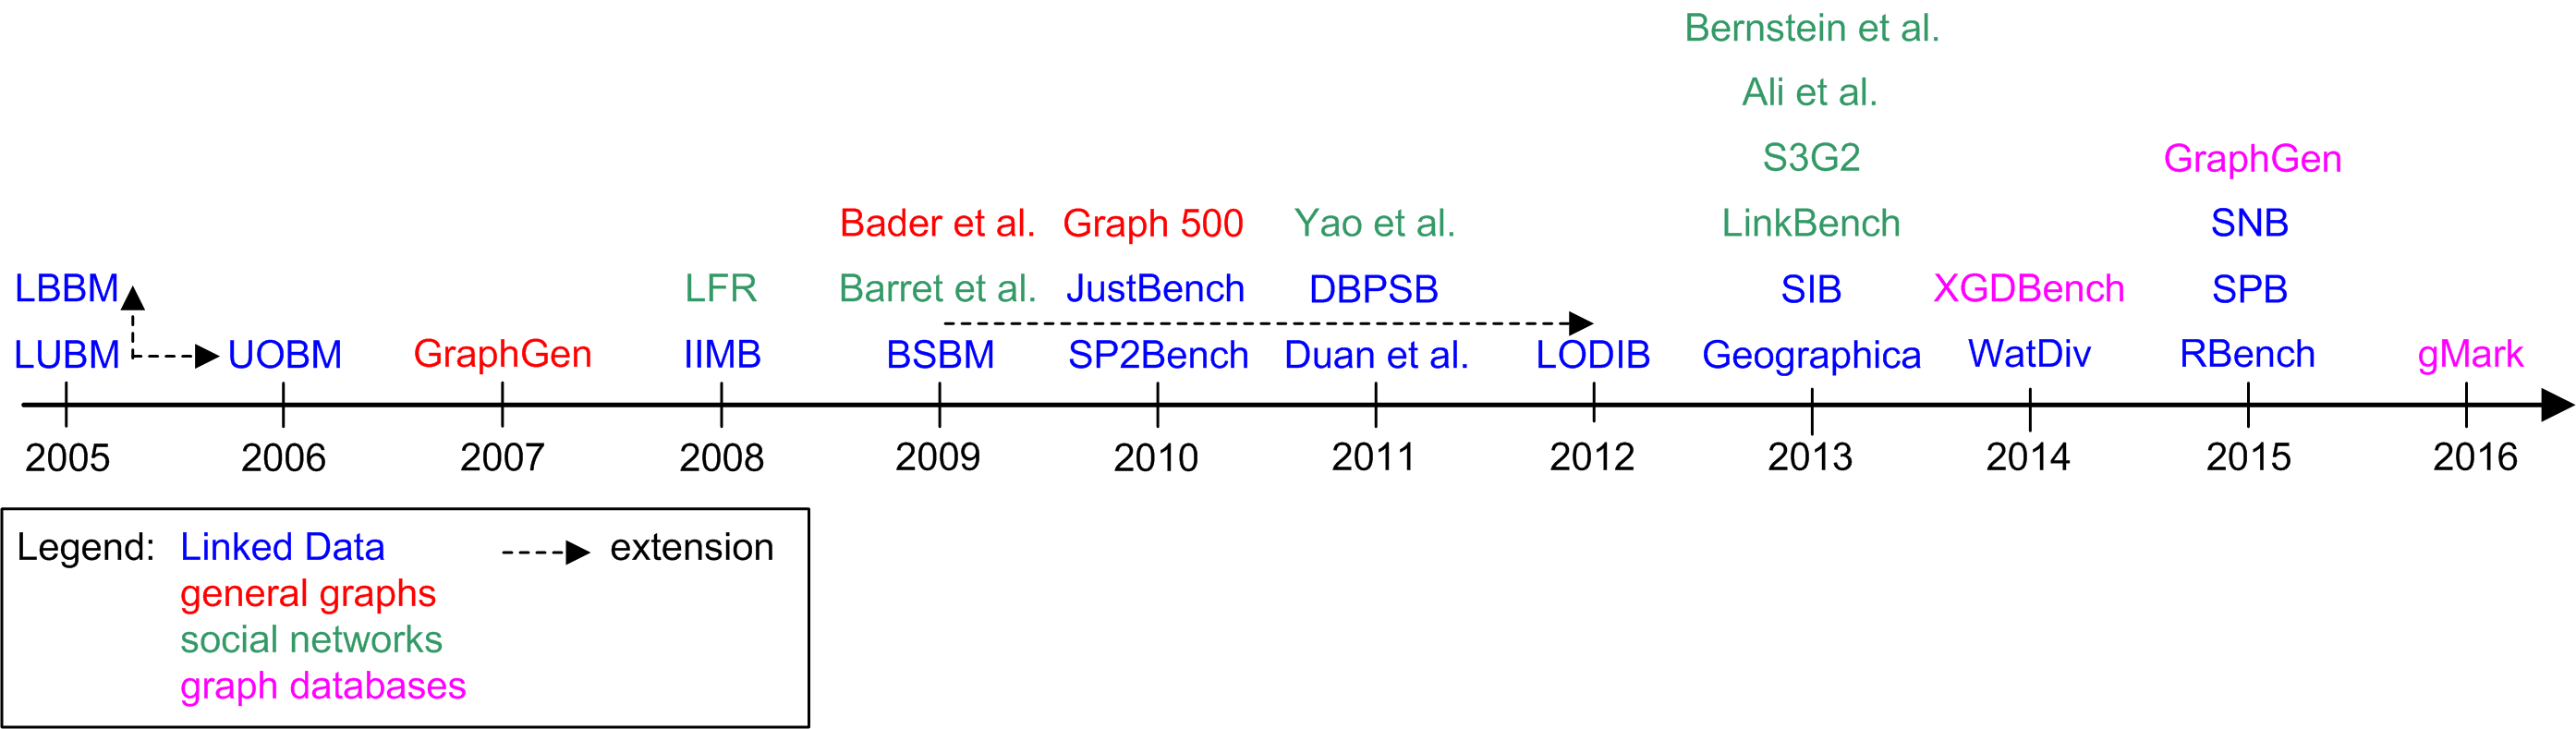
\includegraphics[width=\textwidth]{timeline1.png}
\caption{Timeline}
\label{fig:timeline1}
\end{figure}


Next, in Tables~\ref{tab:comparison_gen_text} to~\ref{tab:comparison_sn_yesno} we compare the functionalities of the generators. We focus on ....

%%%%%%%%%%%%%%%%%%%%%%%%%%%%%%%%%%%%%%%%%%%%%%%

\begin{table}[h]
\footnotesize
\centering
\tbl{Comparison of graph data generators -- general graphs}{
\begin{tabular}{| p{1.9cm} | p{1.2cm} | p{1.5cm} | p{1.3cm} | p{1.5cm} | p{1.5cm} |p{1.5cm} |}
 \hline
               & Graph
               & Parameters
               & Algorithm
               & Output format
               & Operations
               & Problem domain
               \\ \hline \hline
%   &  & & & &   &         \\ \hline
 GraphGen~\cite{GraphGen}   & labelled, undirected, connected & number of graphs, average size of graphs, average density, ... & \NO & list of graphs, their nodes and edges & frequent subgraph mining, query processing  &  \NO       \\ \hline
 HPC Scalable Graph Analysis Benchmark \cite{HPCgraph}  & weighted, directed & number of vertices, number of edges, and maximum weight of an edge & R-MAT & tuples $\langle$ start vertex, end vertex, weight $\rangle$ & classification of large vertex sets, graph extraction with BFS, and graph analysis with betweenness centrality & \NO         \\ \hline
 Graph 500 Benchmark \cite{Graph500} & weighted, undirected & scale, edge factor & R-MAT & tuples $\langle$ start vertex, end vertex, weight $\rangle$ & BFS  & \NO        \\ \hline
\end{tabular} }
\label{tab:comparison_gen_text}
\end{table}

\begin{table}[h]
\footnotesize
\centering
\tbl{Comparison of graph data generators -- Linked Data}{
\begin{tabular}{| p{1.9cm} | p{1.2cm} | p{3cm} | p{1.3cm} | p{3cm} | p{1.5cm} |}
 \hline
               & Graph
               & Parameters
               & Output format
               & Queries
               & Problem domain
               \\ \hline \hline
 LUBM \cite{Guo2005158} & RDF & seed for random number generation, number of universities, starting index of universities & RDF &  14 & storing, querying \\ \hline
 LBBM \cite{Wang2005} & RDF &  number of triples & RDF &  12 & storing, querying \\ \hline
 UOBM \cite{Ma:2006:TCO:2094613.2094629} & RDF & number of universities, probability of generating of various additional links & RDF & 15 & storing, querying  \\ \hline
 IIMB \cite{Ferrara08OM} & RDF & required transformations & RDF & \NO & instance matching \\ \hline
 BSBM \cite{Bizer09theberlin} & RDF & number of products & RDF, relational  & 12 & storing, querying          \\ \hline
 SP$^2$Bench \cite{Schmidt2010} & RDF & triple count / year up to which data is
generated & RDF & 12  &  storing, querying        \\ \hline
 \cite{Duan:2011:AOC:1989323.1989340} & RDF & size, coherence & RDF & \NO    &  storing, querying     \\ \hline
 DBPSB \cite{Morsey2011}     & RDF    & scale factor     & RDF    & 25 derived templates  & storing, querying\\ \hline
 LODIB \cite{DBLP:conf/www/RiveroSBR12} & RDF & number of product instances & RDF & \NO           & translation systems \\ \hline
 SIB \cite{sib} & RDF & number of users & RDF &  3 query mixes    & storing, querying \\ \hline
 Geographica \cite{DBLP:conf/semweb/GarbisKK13} & RDF & size & RDF & 29 + 11 queries + 2 query templates  & geospatial RDF stores    \\ \hline
 WatDiv \cite{Aluc:2014:DST:2717213.2717229}     &  RDF   &  WatDiv schema, scale factor, value distributions, number of query templates, their restrictions  &  RDF   &  user-specified number of query templates and respective query instances & storing, querying \\ \hline
 RBench \cite{Qiao:2015:RAR:2723372.2746479}     &   RDF  &  size + degree scaling factor   & RDF    & 5 types of queries generated for the synthetic data  & storing, querying  \\ \hline
 LDBC SPB \cite{spb}     & RDF   & size     & RDF   & 2 query mixes   & storing, querying \\ \hline
\end{tabular} }
\label{tab:comparison_ld_text}
\end{table}

\begin{table}[h]
\footnotesize
\centering
\tbl{Comparison of graph data generators -- graph databases}{
\begin{tabular}{| p{1.9cm} | p{1.2cm} | p{3cm} | p{1.3cm} | p{3cm} | p{1.5cm} |}
 \hline
               & Graph
               & Parameters
               & Output format
               & Queries
               & Problem domain
               \\ \hline \hline
gMark~\cite{gMark}   & any & graph and query workload configuration & various (e.g., N-triples + SQL, SPARQL, Datalog, openCypher) & synthetically generated  & querying, graph analytics, schema validation         \\ \hline
XGDBench~\cite{Dayarathna:2014:GDB:2676904.2676939}  & any & number of vertices and attributes per vertex, a threshold for random initialization of attributes, an edge affinity threshold, an affinity matrix & DistArray of X10 & 7 workloads & storing, graph operations \\ \hline
\end{tabular} }
\label{tab:comparison_gdb_text}
\end{table}

\begin{table}[h]
\footnotesize
\centering
\tbl{Comparison of graph data generators -- social networks}{
\begin{tabular}{| p{1.9cm} | p{1.2cm} | p{3cm} | p{1.3cm} | p{3cm} | p{1.5cm} |}
 \hline
               & Graph
               & Parameters
               & Output format
               & Queries
               & Problem domain
               \\ \hline \hline
 LFR~\cite{PhysRevE.78.046110}      & social network    & number of nodes, power-law exponents, mixing parameter  & n/a   & \NO    &  community detection    \\ \hline
 \cite{Barrett:2009:GAL:1995456.1995598} & social network & data sets, activity templates & n/a & \NO & analysis        \\ \hline
 \cite{Yao2011}   & linkage graph & burning probability, symmetry probability & n/a & \NO  & degree correlation analysis         \\ \hline
 LinkBench \cite{Armstrong:2013:LDB:2463676.2465296} & social network & number of nodes & MySQL compliant &  10 graph operations  & storing, data access       \\ \hline
 S3G2 \cite{Pham2013} & social network (RDF) & data schema, dictionaries, property value correlations, correlation dimensions  & RDF & \NO & storing, analysis         \\ \hline
 \cite{Sukthankar-SocialInfo2014} & social network & network to be cloned, homophily, link density & n/a & \NO & benchmarking, debugging, simulation   \\ \hline
 LDBC SNB \cite{Erling:2015:LSN:2723372.2742786}     &  social network (RDF)   &  the amount of persons    &  RDF (CSV, Ntriple)   & 3 workloads  &  storing, querying \\ \hline
\end{tabular} }
\label{tab:comparison_sn_text}
\end{table}

%%%%%%%%%%%%%%%%%%%%%%%%%%%%%%%%%%%%%%%%%%%%%%%%%%%%%%%%%%%%%%

\begin{table}[h]
\footnotesize
\centering
\tbl{Comparison of graph data generators -- general graphs (yes/no features)}{
\begin{tabular}{| l | l | l | l | l | l | l | l | }
 \hline
               & \rot{Domain-specific}
               & \rot{Language-specific}
               & \rot{Use-case driven}
               &  \rot{Considering true Big Data}
               \\ \hline \hline
% &  &  &  &            \\ \hline
 GraphGen \cite{GraphGen}  & \NO & \NO & \NO & \OK           \\ \hline
 HPC Scalable Graph Analysis Benchmark\cite{HPCgraph}  & \NO & \NO & \NO & \OK           \\ \hline
 Graph 500 Benchmark \cite{Graph500}     & \NO    &  \NO    & \NO    & \OK    \\ \hline
\end{tabular} }
\label{tab:comparison_gen_yesno}
\end{table}

\begin{table}[h]
\footnotesize
\centering
\tbl{Comparison of graph data generators -- Linked Data (yes/no features)}{
\begin{tabular}{| l | l | l | l | l | l | l | l | }
 \hline
               & \rot{Domain-specific}
               & \rot{Language-specific}
               & \rot{Use-case driven}
               &  \rot{Considering true Big Data}
               \\ \hline \hline
 LUBM \cite{Guo2005158}     & \OK    &  \NO    &  \OK   & \NO     \\ \hline
 LBBM \cite{Wang2005}     & \NO    &  \NO    &   \NO  &  \NO    \\ \hline
 UOBM \cite{Ma:2006:TCO:2094613.2094629}     &  \OK    &  \NO    &  \OK    & \NO     \\ \hline
 IIMB \cite{Ferrara08OM} & \OK & \NO & \OK &  \NO          \\ \hline
 BSBM \cite{Bizer09theberlin}     &  \OK   &  \NO    & \OK    &  \NO    \\ \hline
 SP$^2$Bench \cite{Schmidt2010}     & \OK    &  \OK    & \NO    &  \NO    \\ \hline
 \cite{Duan:2011:AOC:1989323.1989340}     & \NO & \NO  &  \NO   &  \NO    \\ \hline
 DBPSB \cite{Morsey2011}     & \OK    &  \NO    &  \OK   &  \NO    \\ \hline
 LODIB \cite{DBLP:conf/www/RiveroSBR12} & \OK & \NO & \OK &   \NO         \\ \hline
 SIB \cite{sib} & \OK & \OK & \OK &  \NO          \\ \hline
 Geographica \cite{DBLP:conf/semweb/GarbisKK13} & \OK & \OK & \OK & \NO           \\ \hline
 WatDiv \cite{Aluc:2014:DST:2717213.2717229}     &  \OK   & \OK     &  \NO   &   \NO   \\ \hline
 RBench \cite{Qiao:2015:RAR:2723372.2746479}     &  \NO   & \NO     & \NO    & \NO     \\ \hline
 LDBC SPB \cite{spb}     & \OK    & \NO     & \OK    &  \NO    \\ \hline
\end{tabular} }
\label{tab:comparison_ld_yesno}
\end{table}

\begin{table}[h]
\footnotesize
\centering
\tbl{Comparison of graph data generators -- graph databases (yes/no features)}{
\begin{tabular}{| l | l | l | l | l | l | l | l | }
 \hline
               & \rot{Domain-specific}
               & \rot{Language-specific}
               & \rot{Use-case driven}
               &  \rot{Considering true Big Data}
               \\ \hline \hline
Graph 500 Benchmark~\cite{Graph500}     & \NO    &  \NO    & \NO    & \NO     \\ \hline
XGDBench~\cite{Dayarathna:2014:GDB:2676904.2676939}      & \NO    & \NO     &  \NO   & \OK     \\ \hline
%      &     &      &     &      \\ \hline
\end{tabular} }
\label{tab:comparison_gdb_yesno}
\end{table}

\begin{table}[h]
\footnotesize
\centering
\tbl{Comparison of graph data generators -- social networks (yes/no features)}{
\begin{tabular}{| l | l | l | l | l | l | l | l | }
 \hline
               & \rot{Domain-specific}
               & \rot{Language-specific}
               & \rot{Use-case driven}
               & \rot{Considering true Big Data}
               & \rot{Statistical/Agent-based}
               \\ \hline \hline
LFR~\cite{PhysRevE.78.046110}      & \NO    &  \NO    & \NO    & \NO  & S   \\ \hline
 \cite{Barrett:2009:GAL:1995456.1995598} & \NO    &  \NO    & \NO    & \NO  & A   \\ \hline
 \cite{Yao2011}   & \NO  & \NO & \NO  & \NO  & S        \\ \hline
 LinkBench \cite{Armstrong:2013:LDB:2463676.2465296} & \OK & \NO & \OK & \OK & S          \\ \hline
  S3G2 \cite{Pham2013} & \NO & \NO & \NO & \OK & S       \\ \hline
%  \cite{Bernstein:2013:SAS:2499604.2499609} & \NO & \NO & \NO & \OK & A       \\ \hline
 \cite{Sukthankar-SocialInfo2014} & \NO    &  \NO    & \NO    & \NO & S    \\ \hline
 LDBC-SNB \cite{Erling:2015:LSN:2723372.2742786}     &   \OK    & \NO     & \OK    & \OK  & S  \\ \hline
%      &     &      &     &      \\ \hline

\end{tabular} }
\label{tab:comparison_sn_yesno}
\end{table}


As we can see ...

\section{Challenges and Open Problems}
\label{sec:challenges}

To conclude the  overview of the state-of-the-art of graph data generation, in this section we discuss several of the open challenges.

\subsection{Simple Usage, Simple Parameters}
The proposal of a data generator (not necessarily for graph data) has to face an
important schism. On one hand, it must provide the user with as
many parameters as possible in order to enable him/her to generate
arbitrary data.
This approach seems to be reasonable, but it entails a shortcoming due to
the fact that ordinary users are
unwilling to use complex benchmarking tools. This observation can be
seen, for example, in the case of XML benchmarks -- even though there exist
robust and complex data generators (such as
ToXGene~\cite{conf/webdb/BarbosaMKL02}, which supports specification of
structural aspects, value distributions, references etc.), the most popular
benchmarking tool is XMark~\cite{Schmidt:2002:XBX:1287369.1287455}, which models
a single use case and enables to specify just the size of the data. Hence, the
other extreme is to provide a simple data generator which does not require any
complex settings and thus guarantees a simple and fast benchmarking process.

Considering the complex structure of graph data and the variety of applications
requiring highly specific types of graphs, the latter solution is difficult to
implement. A reasonable compromise can be found in a data generator which is
provided with sample graph data and is capable of automatic analysis of its
structural and value features in order to learn the complex parameters.

\subsection{Large Scale Graphs with Realistic Structure}

Most of existing graph generators aiming at generating large graphs with realistic
structural characteristics focus principally on reproducing the degree
distribution and the clustering
coefficient~\cite{kolda2014scalable,edunov2016darwini}. However, there are other
structural characteristics one might be interested in reproducing for a large
graph, such as the diameter, the size of the largest connected component, or the
hierarchical community structure. Graph practitioners are highly interested in knowing
how other high-level structural characteristics affect the performance of graph
queries and graph algorithms. Hence, a compelling open challenge consists
of creating
graph generators that allow to reproduce diverse structural characteristics
of the graphs along with large scale sizes.

\subsection{Single- vs. Multi-domain}

Most of existing graph generators generate graphs that are either not labeled or
are specific to a given domain (e.g.  Social Networks). Graphs from different
domains have different schemas, structural characteristics, property
distributions, etc. which might have an impact on the performance of the
application under test. Thus, graph processing engine developers are asking for
generators or tools to flexibly and holistically generate multi-domain graphs, allowing to configure aspects
such as size, schemata, data distributions and other structural
characteristics such as degree distributions, clustering coefficients, and
so on.

\subsection{Generating Noisy Graphs and Graphs with Anomalies}
Injecting noise and/or anomalies and errors into graphs is crucial for
testing both machine learning algorithms working on this complex data and
data quality techniques aiming at detecting anomalies and repairing graph
data.

Concerning the former, analyzing and labelling structural networks is
deemed to be more difficult for graph datasets in the presence of noise.
Since denoising graph data is difficult to achieve, several machine learning
techniques have been adapted to work with noise (i.e. mislabeled
samples) or outliers, such as
imbalanced graph classification \cite{PanZ13} and
binary graph classification with positive and negative weights \cite{CheungSML16}.
Synthetic graph generators that take into account noisy and missing data
have been studied in \cite{NamataG10}, where graph identification is presented in
order to  model the inference of a cleaned output network from a
noisy input graph.
Concerning the latter, data quality techniques handling graph data are recently considering ad-hoc
generation of graph data and graph quality rules in order to assess the
effectiveness of error detection and data repairing algorithms \cite{FanWX16a,AriouaB18}. The
corresponding graph quality rules are typically handcrafted by domain
experts, whereas an automatic generation of such rules along with the graph
data generation in tandem would be an interesting future challenge for the
community.

\subsection{Streaming Graph Generators}
Stream computing is a new paradigm that is necessitated by various modern data generation scenarios such as the ubiquity of mobile devices, location services,
sensor pervasiveness and emerging IoT applications. These applications generate the data with high Velocity, one of the main 3V characteristics of big data applications~\cite{sakr2016big}. In most of these high speed data generation scenarios, various objects are connected together with different relations and data exchanges  in a graph-structured manner. The Semantic Web community has been considering the aspect of implementing streaming RDF generator and benchmarks, however, there is still a clear lack on considering this aspect in other important and timely domains such as IoT. %Thus, there is a crucial need to tackle this aspect.
In addition, graph streaming generators should  consider some specific aspects for the stream processing domains such as the out-of-order handling (late arrivals)~\cite{li2008out} and the variety in the schemas and formats of the different data streaming sources. It is also recommended for the streaming graph generators to support the distributed environment as this is the most common scenario for such type of applications.

\subsection{Evolving Graph Data}
As user requirements as well as environments change, most of the existing
applications naturally evolve over time, at least to some extent. This evolution
usually influences the structure of the data and consequently all the related
parts of the application (i.e., storage strategies, operations, indexes etc.).
In the world of graph data such graphs that change with time are denoted as \emph{evolving}, \emph{temporal}, \emph{dynamic}, or \emph{time-varying}. They can be modelled as labeled graphs, where the labels capture some measure of time~\cite{Michail2015}.

The evolution of graphs can be considered variously. We can assume a static set of nodes and a varying set of edges.  Or, there are applications where the graphs only ``grow'', i.e., the set of nodes and/or edges is only extended with new items. In the most general case we can assume any changes in both set of nodes and set of edges. Anyway with the evolution aspect the complexity of classical graph problems increases significantly~\cite{Michail2015,Wu:2014:PPT:2732939.2732945}. In some graph applications, such as, e.g., social networks, the evolution of the
data is a significant aspect, especially in the activity graphs~\cite{doreian1997evolution,Kumar:2006:SEO:1150402.1150476,Hellmann2014583,wang2013,Kossinets88,Viswanath:2009:EUI:1592665.1592675}.
However, as shown in~\cite{Leskovec:2005:RMT:2101235.2101254,Leskovec:2005:GOT:1081870.1081893},
evolving graphs have further specific features. For example, some graphs grow over time according to a \emph{densification power law} which means that real graphs tend to sprout many more edges than nodes, and thus are densifying as they grow. Also the effective diameter of graphs tends to shrink or stabilize as the graph grows with time.

A related problem is \emph{data versioning} and respective ability to query across multiple versions of data or to carry out general analysis.
%Considering graph
%data this problem is also common, for example  in the area of Linked
This problem has been investigated for instance within the domain of Linked
Open Data~\cite{DBLP:conf/semweb/Papakonstantinou16,DBLP:conf/esws/MeimarisP16,fernandez2015towards,fernandez2015bear}.


The respective data generator should hence be able to simulate a natural growth and/or changes in the structure of the graph with regards to the various features of distinct use cases. However,  even though the area of dynamic graphs is intensively studied, surprisingly there seem to exist only very few proposals of a generator dealing with this area. In~\cite{GoerkeKlugeSchumm2012_1000029825} the authors focus on \emph{clustering dynamic graphs}, i.e. graphs where the clustering corresponds to the partition of nodes into natural groups based on the paradigm of intra-cluster density versus inter-cluster sparsity of edges. The generator generates a time series of random graphs $G_0, G_1, ..., G_n$, where $G_t$ emerges from $G_{t-1}$ via atomic updates, i.e., insertion or deletion of an edge or a vertex. The generator keeps track of a (dynamic) ground truth clustering. The probability of atomic events is chosen in a way that adheres to this clustering, without losing randomness.

Another recent proposal of a generator~\cite{mlg2018_42} of temporal graphs results from an observation that small subgraph patterns in networks, called \emph{network motifs} or \emph{graphlets}, are crucial indicators of the structure and the evolution of the graphs~\cite{Paranjape:2017:MTN:3018661.3018731}. For a given graph and a predefined ordered list of structural atomic motifs the generator first computes the distribution of the motifs in the graph. The distribution is then used to generate a synthetic graph with the same features.


%\paragraph{} Following the same recursion idea,
%paper~\cite{Leskovec:2005:RMT:2101235.2101254} uses Kronecker multiplication to
%generate self-similar graphs. The network starts with an initial graph G1 that
%contains $N_1$ nodes and $E_1$ edges. Using matrix recursion, larger successive
%graphs $G_2, G_3, ... G_n$ are generated. The $k$-th graph $G_k$ contains $N_k
%= N^k_1$ nodes. Many graphs often densify over time, exhibiting a growth in the
%number of edges that is superlinear to the number of nodes. Kronecker
%multiplication produces graphs with a fixed diameter and a densification power
%law degree distribution with exponent $k = log(E_1)/log(N_1)$. The graph
%generation process introduces a staircase effect in the nodes' degrees, and
%each community consists of smaller nested communities that are formed through
%expansion and recursion.


\subsection{Multi-model Data}
With the dawn of Big Data and especially its variety aspect, new types of
database management systems have emerged. One of the most interesting ones
are the so-called \emph{multi-model databases} that enable to store and
thus query across structurally different data. There exist various types of
multi-model systems combining  distinct subsets of Big Data structures including graph data.
For example, OrientDB\footnote{\url{http://orientdb.com/orientdb/}} which was
implemented on the basis of an object DBMS currently supports graph, document,
key/value, and object models. Such type of DBMSs also needs a specific
data generator that would enable
to test new features and analyze efficiency of operations. However, since the
multi-model systems are in the context of Big Data rather new, there exist only
a few benchmarks targeting multi-model DBMSs (such as
Bigframe~\cite{journals/pvldb/KunjirKB14} or UniBench~\cite{conf/cidr/lu17})
with limited capabilities.


Another interesting approach to multi-model data is to adopt a unifying
expressive graph data model, known as property graph data
model~\cite{BFVY18}. Such a model allows to specify multi-edges and list of
properties for the nodes. Synthetic graph generators for property graphs and its
companion standard graph query language~\cite{Angles18,AnglesABBFGLPPS18} are also needed in order to boost
their availability and adoption for different communities.


\subsection{Machine Learning Based Graph Generation}

With the advent of neural networks and specially generative adversarial networks
(GANs)~\cite{goodfellow2014generative}, several researchers have started to
explore their application to generate graphs. This is the case of
~\cite{kipf2016variational,grover2018graphite,simonovsky2018graphvae,li2018learning,you2018graphrnn},
which present several generative models to generate realistic graphs.  Such
techniques still suffer from several problems. For instance, some of them are
limited to learn from a single
graph~\cite{kipf2016variational,grover2018graphite} or generate small
graphs~\cite{simonovsky2018graphvae,li2018learning,you2018graphrnn}. The
technique proposed in~\cite{you2018graphrnn} is capable of generating graphs
with complex edge dependencies (e.g. community structure) and is not restricted
to graphs of a fixed size. However, there are still in general several open
challenges, including the capability of learning from and generating large graphs comparable
in size to those typically used for benchmarking, and robust generation
techniques with structural guarantees (e.g. degree distribution, clustering
coefficient, etc.).

\subsection{Privacy-preserving Graph Generation}

A lot of work has been conducted on techniques for publishing social network
graphs with privacy guarantees~\cite{wu2010survey}. However, the topic of
generating social graphs with a realistic structure yet private has been barely explored.  

Most of the existing work falls within the topic of graph generation with ``differential
privacy''~\cite{dwork2009differential} guarantees. More specifically, in
~\cite{wang2013preserving} the authors develop a differential privacy graph
generation approach based on the dK-graph generation
model~\cite{mahadevan2006systematic} that outperforms the Stochastic Kronecker
Graph Model~\cite{LeskovecCKF05} in terms of the produced structural properties,
eventhough the results show that there is still room for improvement.

Following this line of research, recent work~\cite{qin2017generating} extends the notion of differential privacy
and propose an `` edge local differential privacy'' based graph generation
method. The poposed method allows generating privacy preserving synthetic social
graphs wihtout the need of a centralized data curator, while preserving structural
properties more accurately than straw-hat methods such as Randomized
Neighbor Lists (based on randomized response~\cite{dwork2014algorithmic}) and
Degree-based Graph Generation (which perturbates the original graph degrees
using the Laplace mechanism~\cite{dwork2009differential}). Again, eventhough the
proposed technique outperforms the baselines, the results show that there is
still room for improvement in terms of the structural properties of the
generated graph.

\section{Conclusion}
\label{sec:conclusion}


... 


\begin{acks}
The authors would like to thank Dr. Kamesh Madduri for numerous consultations and suggestions on the covered areas.
\end{acks}

% Bibliography
\bibliographystyle{ACM-Reference-Format-Journals}
\bibliography{biblio}

% History dates
\received{August 2016}{September 2016}{December 2016}


\end{document} 